\documentclass[a4paper,12pt,english,final]{epsc_tfc_pfc}
%% a4paper: mida paper. No tocar
%% 12pt: mida de la font. No tocar

%%  - OPCIONS A CONFIGURAR:
%%     - Estat del document: final o draft
%%       NOTA: Draft no inserta les figures i indica quan el text sobrepassa els marges.

%%  - IDIOMES QUE S'USARAN EN EL DOCUMENT: catalan, spanish, english, french...
%%    NOTA: per canviar d'idioma al mig del document usar:
%%          \selectlanguage{nom_idioma}
\usepackage[english,catalan]{babel}

%%%%%%%%%%%%%%%%%%%%%%%%%%%%%%%%%%%%%%%%%%%%%%%%%%%%%%%%%%%%%%%%%%%%%%%%%%%%%


%%% PAQUETS LATEX RECOMANABLES A UTILITZAR
%%%%%%%%%%%%%%%%%%%%%%%%%%%%%%%%%%%%%%%%%%%%%%%%%%%%%%%%%%%%%%%%%%%%%%%%%%%%%
%%% NOTA: es possible que algunes distribuicions Linux o Windows 
%%%       no portin aquests paquets instal�lats per defecte.

%% El paquet isolatin1 �s extramadament �til. 
%% Permet escriure els accents directament amb l'editor de texte
%% sense haver de fer coses com per exemple: introducci\'o
\usepackage[latin1]{inputenc}             

%% S�mbols matem�tics de la American Mathematical Society
\usepackage{amssymb,amsmath,amsfonts}

\usepackage{titlesec}

%% Glossaries
%\usepackage[nonumberlist,section=chapter]{glossaries}
\usepackage{glossaries}
\makeglossaries

%% El paquet array proporciona eines molt �tils a l'hora de fer 
%% equacions amb matrius
\usepackage{array}             

%% Permet fer taules fusionant cel�les de files consecutives
%\usepackage{multirow}          

%% Permet canviar els colors del document
%\usepackage{color,colortbl}
\usepackage{float}

\restylefloat{table}

\usepackage{textcomp}

\usepackage[export]{adjustbox}

\usepackage{times}

%\url
\usepackage{url}

\begin{document}
\pagestyle{empty}
%%%%%%%%%%%%%%%%%%%%%%%%%%%%%%%%%%%%%%%%%%%%%%%%%%%%%%%%%%%%%%%%%%%%%%%%%%%%%
%%%%%%%%%%%%%%%%%%%%%%%%%%%%%%%%%%%%%%%%%%%%%%%%%%%%%%%%%%%%%%%%%%%%%%%%%%%%%

%% IDIOMA PRINCIPAL DEL DOCUMENT
%%%%%%%%%%%%%%%%%%%%%%%%%%%%%%%%%%%%%%%%%%%%%%%%%%%%%%%%%%%%%%%%%%%%%%%%%%%%%
\selectlanguage{english}

%%%%%%%%%%%%%%%%%%%%%%%%%%%%%%%%%%%%%%%%%%%%%%%%%%%%%%%%%%%%%%%%%%%%%%%%%%%%%
%% PORTADA
%%%%%%%%%%%%%%%%%%%%%%%%%%%%%%%%%%%%%%%%%%%%%%%%%%%%%%%%%%%%%%%%%%%%%%%%%%%%%
%% Portada generada autom�ticament a partir del fitxer de dades
\portada

%% RESUM
%%%%%%%%%%%%%%%%%%%%%%%%%%%%%%%%%%%%%%%%%%%%%%%%%%%%%%%%%%%%%%%%%%%%%%%%%%%%%
% NOTA: la longitud passada com a parametre d'entrada 
%       s'ha d'ajustar ``a ull'' fins que el requadre del resum ocupi tota la pagina 
\begin{resum}{10cm}
Aquest document cont� les pautes del format de presentaci� del treball o projecte de final de carrera. En tot cas, cal tenir en compte el que estableix la ``Normativa del treball de fi de carrera (TFC) i del projecte de fi de carrera (PFC)'' aprovada per la Comissi� Permanent de l'EPSC, especialment l'apartat ``Requeriments del treball''.
\end{resum}

%% OVERVIEW
%%%%%%%%%%%%%%%%%%%%%%%%%%%%%%%%%%%%%%%%%%%%%%%%%%%%%%%%%%%%%%%%%%%%%%%%%%%%%
% NOTA: la longitud passada com a parametre d'entrada 
%       s'ha d'ajustar ``a ull'' fins que el requadre del resum ocupi tota la pagina 
\begin{overview}{11cm}
This document contains guidelines for writing your TFC/PFC. However, you should also take into consideration the standards established in the document Normativa del treball de fi de carrera (TFC) i del projecte de fi de carrera (PFC), paying special attention to the section Requeriments del treball, as this document has been approved by the EPSC Standing Committee
\end{overview}

%% DEDICATORIA (opcional)
%%%%%%%%%%%%%%%%%%%%%%%%%%%%%%%%%%%%%%%%%%%%%%%%%%%%%%%%%%%%%%%%%%%%%%%%%%%%%
\begin{dedicatoria}
Escriure aqu� opcionalment la dedicat�ria.
\end{dedicatoria}

%% INDEX de continguts
%%%%%%%%%%%%%%%%%%%%%%%%%%%%%%%%%%%%%%%%%%%%%%%%%%%%%%%%%%%%%%%%%%%%%%%%%%%%%
\thispagestyle{empty} 
\tableofcontents
\cleardoublepage

%% INDEX de figures (opcional, comentar les 3 linies si no es desitja)
%%%%%%%%%%%%%%%%%%%%%%%%%%%%%%%%%%%%%%%%%%%%%%%%%%%%%%%%%%%%%%%%%%%%%%%%%%%%%
\thispagestyle{empty}
\listoffigures
\cleardoublepage

%% INDEX de taules (opcional, comentar les 3 linies si no es desitja)
%%%%%%%%%%%%%%%%%%%%%%%%%%%%%%%%%%%%%%%%%%%%%%%%%%%%%%%%%%%%%%%%%%%%%%%%%%%%%
\thispagestyle{empty}
\listoftables
\cleardoublepage

%%%%%%%%%%%%%%%%%%%%%%%%%%%%%%%%%%%%%%%%%%%%%%%%%%%%%%%%%%%%%%%%%%%%%%%%%%
%%%%%%                    INTRODUCCI�                          %%%%%%%%%%%
%%%%%%%%%%%%%%%%%%%%%%%%%%%%%%%%%%%%%%%%%%%%%%%%%%%%%%%%%%%%%%%%%%%%%%%%%%
%% NOTA: El text passat com a parametre d'entrada 
%%       �s ''introducci�'' amb l'idioma en que es redacti el projecte
\pagestyle{fancy} 

%% First include Glossary to be used in the following chapters
%% INDEX de glossari
%%%%%%%%%%%%%%%%%%%%%%%%%%%%%%%%%%%%%%%%%%%%%%%%%%%%%%%%%%%%%%%%%%%%%%%%%%%%%\\
\thispagestyle{empty}
\newglossaryentry{SoC}{name={SoC},description={System-on-Chip}}
\newglossaryentry{ISM}{name={ISM},description={Industrial, Scientific and Medical}}
\newglossaryentry{GPIO}{name={GPIO},description={General-purpose input/output}}
\newglossaryentry{SPI}{name={SPI},description={Serial Peripheral Interface}}
\newglossaryentry{IRQ}{name={IRQ},description={Interrupt Request}}
\newglossaryentry{BCM2835}{name={BCM2835},description={ARMv6 CPU mounted on the RaspberryPi}}
\newglossaryentry{FD}{name={File Descriptor},description={file descriptor (FD) is an abstract indicator for accessing a file on \gls{POSIX} systems}}
\newglossaryentry{POSIX}{name={POSIX},description={Portable Operating System Interface. X stands for Unix}}
\newglossaryentry{SYSFS}{name={SYSFS},description={Virtual file system provided by Linux. SYSFS exports information about devices and drivers from the kernel device model to user space}}
\newglossaryentry{PWM}{name={PWM},description={Pulse-width modulation}}
\newglossaryentry{UART}{name={UART},description={Universal Asynchronous Receiver/Transmitter}}
\newglossaryentry{IOCTL}{name={ioctl},description={Abbreviation of input/output control, system call used for device-specific input/output operations}}
\newglossaryentry{MISO}{name={MISO},description={Master Input Slave Output}}
\newglossaryentry{MOSI}{name={MOSI},description={Master Output Slave Input}}
\newglossaryentry{SCLK}{name={SCLK},description={Serial Clock}}
\newglossaryentry{CS}{name={CS},description={Chip Select}}
%\printglossaries
%\cleardoublepage

\begin{intro}{Introduction} 
Embedded systems have become more powerful over time passing from 8 bit controllers to 8 or 16 bit microprocessors or even 32 bit ARM microprocessors, apart from the increase of the processing power, the memory included in this devices is also increased, from  tens of Kilobytes to tens or hundreds of Megabytes. One of the reasons for this changes has been the price drop on production. This new embedded systems offers a power similar to the computers from the nineties and most of them implement operating systems which this helps on reducing the difficulty to create embedded applications. With an operating system running over the bare metal of the chip, the developer will get all the underlying hardware abstracted to different APIs and libraries and avoiding low level interaction with the hardware. They also offer interesting features such as memory control and allocation, threading, dynamic program loading. In example, one of the top notch devices nowadays is the Raspberry Pi which mounts an ARM6, 512MB of RAM and some I/O features such as GPIOs, SPI, UART. This hardware can be equivalent to a nineties computer similar to a Pentium II so they are really powerful to the task that they may do.
\\
One of the operating systems for embedded devices is .NET Micro Framework (NETMF) developed by Microsoft. This system is the smallest version of .NET Framework and is oriented to resource-constrained devices for embedded applications. This system offers different communication protocols and methods like the \gls{GPIO} ports, the \gls{SPI}, \gls{UART} and \gls{I2C}. There is no official implementation or port of Micro Framework that is capable to run on standard computers (a normal desktop), so any application written for this operating system will not work on Linux or Windows, and although exists a minimal port of this system to a Linux board called Eddy it do not offers all the hardware features that Micro Framework do, and it is only focused to the named board.
\\
The aim of IOSharp is solve this lack and get Micro Framework applications run on any Linux machine which is capable of running applications using the .NET Framework (the complete stack designed by Microsoft). So this project instead of writing a complete port of the Micro Framework runtime to run on Linux is an extension to the classes provided by the .NET Framework. Basically IOSharp offers the IO functions, methods and classes that are missing on .NET Framework, and although the implementation of the classes is different in IOSharp than in Micro Framework, the namespaces, methods, class naming, etc is equal to the original ones so this makes much easy to migrate between Micro Framework to .NET Framework. 
\\
The reason for this implementation is try to migrate the Micro Framework code that runs on a Netduino Mini which is the gateway of a Wireless Sensor Network (\gls{WSN}). One of the problems that this platform has is that the it is getting out of system resources, so in order to keep the existing code different solutions are being researched, in this case IOSharp pretends to be one of that solutions achieving the deployment of this WSN gateway software on a Raspberry Pi which runs a Linux operating system.
\\
\\
After achieving the first goal, there is a second expansion project which consists of extending a code translating tool called AlterNative which is being developed by Alex Albal� and Juan L�pez. This translator is capable to get the source code from a C\# binary and then translate it to C++ trying to get better performance than C\#. C++ theoretically performs better than C\# applications, but normally are more platform oriented, so Windows binary will not work on a Linux sytem, but one of the interesting features of AlterNative is generate a highly portable code that can be compiled on (and for) any operating system, i.e. Windows, Linux, MacOSX, iOS, Android, etc. Another interesting point of this tool is that the generated code is similar to C\# so a developer used to this language will be able to understand or even write programs using the translated code.

\end{intro}

\pagestyle{fancy} 

%%%%%%%%%%%%%%%%%%%%%%%%%%%%%%%%%%%%%%%%%%%%%%%%%%%%%%%%%%%%%%%%%%%%%%%%%%
%%%%%% INCLOURE A PARTIR D'AQU� TOTS ELS CAP�TOLS DE LA MEMORIA   %%%%%%%%
%%%%%%%%%%%%%%%%%%%%%%%%%%%%%%%%%%%%%%%%%%%%%%%%%%%%%%%%%%%%%%%%%%%%%%%%%%

%% First include Glossary to be used in the following chapters
%%% INDEX de glossari
%%%%%%%%%%%%%%%%%%%%%%%%%%%%%%%%%%%%%%%%%%%%%%%%%%%%%%%%%%%%%%%%%%%%%%%%%%%%%\\
\thispagestyle{empty}
\newglossaryentry{SoC}{name={SoC},description={System-on-Chip}}
\newglossaryentry{ISM}{name={ISM},description={Industrial, Scientific and Medical}}
\newglossaryentry{GPIO}{name={GPIO},description={General-purpose input/output}}
\newglossaryentry{SPI}{name={SPI},description={Serial Peripheral Interface}}
\newglossaryentry{IRQ}{name={IRQ},description={Interrupt Request}}
\newglossaryentry{BCM2835}{name={BCM2835},description={ARMv6 CPU mounted on the RaspberryPi}}
\newglossaryentry{FD}{name={File Descriptor},description={file descriptor (FD) is an abstract indicator for accessing a file on \gls{POSIX} systems}}
\newglossaryentry{POSIX}{name={POSIX},description={Portable Operating System Interface. X stands for Unix}}
\newglossaryentry{SYSFS}{name={SYSFS},description={Virtual file system provided by Linux. SYSFS exports information about devices and drivers from the kernel device model to user space}}
\newglossaryentry{PWM}{name={PWM},description={Pulse-width modulation}}
\newglossaryentry{UART}{name={UART},description={Universal Asynchronous Receiver/Transmitter}}
\newglossaryentry{IOCTL}{name={ioctl},description={Abbreviation of input/output control, system call used for device-specific input/output operations}}
\newglossaryentry{MISO}{name={MISO},description={Master Input Slave Output}}
\newglossaryentry{MOSI}{name={MOSI},description={Master Output Slave Input}}
\newglossaryentry{SCLK}{name={SCLK},description={Serial Clock}}
\newglossaryentry{CS}{name={CS},description={Chip Select}}
%\printglossaries
%\cleardoublepage

%% Include the chapters
\chapter{Project overview}\label{C:project-overview}
This project was proposed by AlterAid a company which is working on several ways to help in taking care of the health of our elderly, or in general, anyone that is relevant to our lives.

This company is working on two different projects that combine together, the first one is called aaaida which consists of a social network where people can stay alert about its relatives, upload information about its health or watch recommendations from doctors or other professionals. On the other side, and more hardware oriented development, they are creating a Sensor Network called HomeSense that once deployed in a house will be able to collect relevant information from those sensors in the home and allow other people to know if the daily life of the resident's house is going normal, or something is happening.

\section{AlterAid products in depth}\label{S:alteraid-products}
%As explained before, AlterAid has two relevant products, aaaida which is the unifying social network that shows or even analyzes the data uploaded there. Then comes HomeSense, a Wireles Healthcare Sensor Platform, which is interesting on terms of sensing and daily life control. HomeSense idea is be able to gather information by using distributed sensors around a house and then upload this information to aaaida.

\subsection{HomeSense}\label{SS:HomeSense-proposal}
HomeSense, is a Wireless Healthcare Sensor Platform \gls{WSN} created with the aim of control and care taking of the elderly and relatives, actually it uses a Netduino board which makes the function of the gateway which controls the sensor network, receiving all the data and uploading to aaaida platform through internet.
\\
In the house the communication is carried on using little sensors capable of fetching data in different situations for example a drawer or a medicine cabinet, it is also possible to install the sensors on doors in order to know if they are opened or closed or in any place where is interesting to acquire information from the environment, house or residents. This sensors make use of nRF24LE1 \gls{SoC} with a low-power RF \gls{ISM} band on 2.4GHz from Nordic Semiconductor.
\\
The communication protocol designed for HomeSense is similar to a mesh network with multi-hop transmissions which normally the nodes try to fetch the gateway because this is on charge of upload the information straight to the internet.
\\
The gateway system has been entirely developed using .NET Micro Framework and deployed on a Netduino Mini. The mesh protocol has been defined internally on the company while it uses third-party hardware to create the physical links of the network.

\subsection{Case of use}\label{SS:Case-Of-Use}
Alice is a young teenager whose grandfather, Bob, is ill and she wants to know if all is fine in Bob's home life. Alice will sign up in http://www.aaaida.com, there she will create a bond called Bob. A bond is a entity that represents a person, this entity can be configured with different measures. Then Alice will create 2 measures, the first one will be blood pressure while the other one will be bob's house.
In blood pressure, Bob will use a simple elderly-oriented mobile application in order to upload his blood pressure every day, in this manner Alice can be aware of its health.
Apart from this, Alice will buy a product from AlterAid, called HomeSense, which consists of a set of sensors that must be installed in doors, walls, drawers..., a small centralized system that must be plugged to the power and an application to configure HomeSense.
This application will facilitate the linking between Alice account and Bob's bond, in addition, Alice will be able to setup a internet link to HomeSense using grandfather's Internet or a GSM connection to some mobile phone provider.
Once the system is configured and working, Alice will be able to take care of Bob's home life, for example if he must take a pill at the morning, she can control at least if the medicine cabinet has been opened. Or if all doors are closed if Bob is out of home.

\begin{figure}[H]\begin{center}
 \centering
  \captionsetup{justification=centering}
  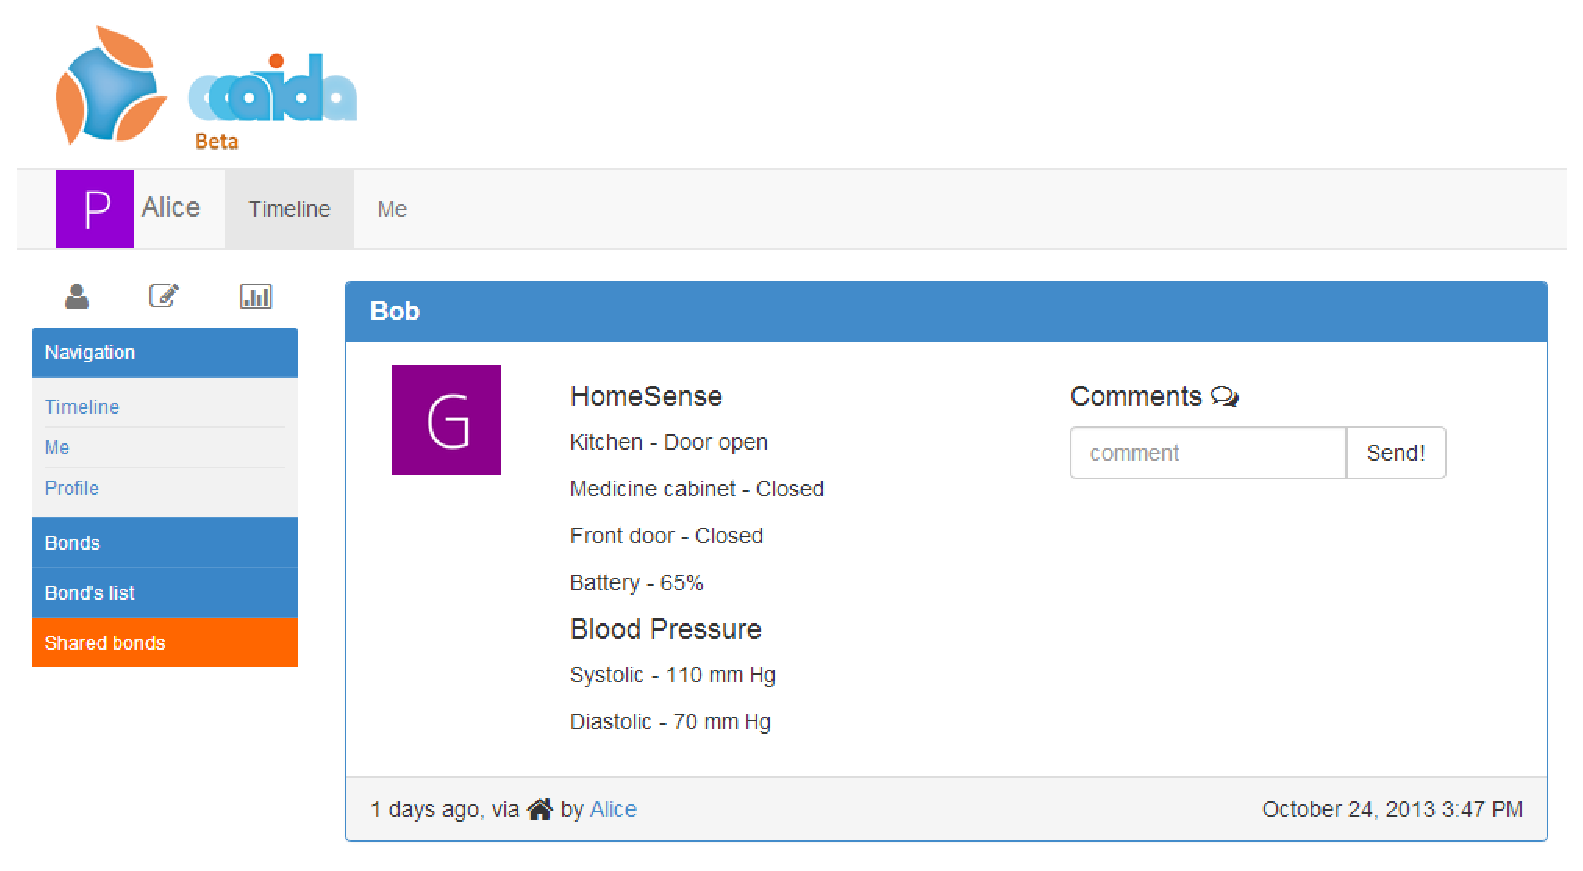
\includegraphics[width=1\textwidth]{pictures/proposal/aaaida-use-case}
  \caption{Case of use representation in aaaida \label{fig:network-architecture}}
\end{center}\end{figure}

\section{AlterNative}\label{S:Proposal-AlterNative}
AlterNative is a language translating tool created by Alex Albal\'{a} and Juan L\'{o}pez. It is capable of translated a compiled (in .NET) binary or library to standard C++ source, basically this program decompiles the the file to be translated, then it sketches how the program works, which are its classes, functions, nodes, etc and then start translating step-by-step all the program, basically it starts writing plain text files with the C++ syntax. After that it links the necessary C++ libraries to work, ones are from boost library, and the other ones are self-written to look like the original C\# classes.
\\
It is interesting to emphasize that the main difference of this translator between the other existing ones is that it tries to generate a code practically identical to the original C\# source code. By doing this, the resulting C++ source is really easy to read for people not used to C++ syntax and language.

\section{Thesis Proposal}\label{S:Proposal-Thesis-Proposal}
After introducing HomeSense and AlterNative is time to explain the thesis proposal itself because it is related to the applications mentioned above. The idea is to take the HomeSense code which runs on closed systems capable of execute a specific .NET framework called Micro Framework, the problem is that the gateway device that runs HomeSense is getting limited in terms of capabilities, performance and expansion for future characteristics.
\\
The idea is to take the gateway code and port it to other devices capable of use minimum GPIO, Interruptions from this ports, the SPI communication protocol and UART because all of them are used in the HomeSense source code. It is important to point that the port must be done on the underlying code which executes Micro Framework code so the original source code should be used without major changes, minor changes such as port renaming and communication module name changing are acceptable because do not alter the original execution flow and design architecture. But not only this should be done on HomeSense, it is interesting to make portable between different hardware platforms any code that runs over Micro Framework.
\\
After accomplishing with this first goal, the second part of the thesis is use AlterNative to translate the IOSharp driver to C++ in order to increase and analyse the performance of IOSharp running on C++ instead of C\#. To accomplish with this some C++ libraries will be need to be written in order to translate IOSharp.
\chapter{State of the art}\label{C:State-Art}

This chapter sketches out briefly the state of the art of the embedded operating systems and its capabilities. Then according to this thesis will be explained what is the current operating system running on the bottom of HomeSense and finally why has been chosen the RaspberryPi as the target device of this thesis.

\section{Embedded Systems}\label{S:Embedded-Systems}
Embedded Systems now a days are taking relevance again with the Internet of the Things, environment sensing, Wireless Sensor Networks and all the coming technologies that require low power consumption, small size, mobility environments etc.

In Embedded Systems or Resource Constrained System it's interesting to take a look into the Hardware platform and its capabilities, and nowadays it 


An operating system (OS) offers an interface with the hardware to make it independent from the applications that the device runs, making easy the interactions between hardware or other running programs.

An OS is an important program that makes easy to develop applications, but it is important to maintain the features that the processor offers, avoiding performance or capabilities degradation. As this bachelor thesis is focused on constrained-resource devices, where the processing capabilities and memory resources are limited, is fundamental to respect the above criteria.

In general, there are three types of operating system architectures based on how applications are executed:

\begin{itemize}
\item \textbf{Monolithic:} The OS and the applications are combined in a single program, being an end to end task without the possibility to include new functions without rewriting much of the code.

\item \textbf{Modular:} The OS is running as a standalone program in the processor and has de ability to load programs to it self as modules. In terms of the development, it's possible to develop applications without writing in the core of the OS.

\item \textbf{Virtual-Machine:} The OS creates an abstraction layer of its underlying hardware, this abstracted layer is common in every device that implements that virtual-machine. Using this type of operating system provides a helpful tool to achieve the well known slogan \textit{write once, run anywhere}. 
\end{itemize}


\begin{itemize}
\item \textbf{TinyOS:} asdf asdf asdf.

\item \textbf{FreeRTOS:} asdf asdf asdf.

\item \textbf{uC/OS II:} asdf asdf asdf.

\item \textbf{Contiki:} asdf asdf asdf.

\item \textbf{Micro Framework .NET:} asdf asdf asdf.
\end{itemize}



\section{Micro Framework .NET}\label{S:MicroFramework}

Complexity and heterogeneity drawbacks of distributed systems could be solved or relived using a middleware. Middleware is a system software that resides between the applications and the underlying operating systems, network protocol stacks, and hardware, which provides facilities in order to build and use distributed systems \cite{cite:middleware}.

This type of software provides a transparent and abstract vision of the low-level details (e.g. network communication, encoding, concurrency, protocol handling, etc.) facilitating end user programming. Middlweware typically provides two different types of transparency to distributed systems:

\begin{itemize}
\item \textbf{Access transparency:} Hides differences between remote and local operations like data representation and invocation mechanisms.

\item \textbf{Location transparency:} Hides where the components reside. The  different components could be 
redistributed (e.g. moved between computers) without changing any of the other components.
\end{itemize}

\subsection{NETMF enabled devices}\label{SS:MicroFramework-Devices}

MicroFramework can run on CLR enabled devices that are MicroFramework compilant with it's specifications. In this bachelor thesis a Netduino Plus (from XXXXXLabs) has been used to test, understand and code sample code in order to know how Microframework works. Apart from this Netduino there are other devices like the cerbuino,which are also capable to run CLR code.

Among this, there are more powerful devices that can run and execute simple graphics programs.


\subsection{Software Development Kit}\label{SS:MicroFramework-SDK}
As Micro Framework is similar to an operating system it has

\begin{itemize}
\item \textbf{4.3:} This asynchronous indirect communication model uses a queue in order to exchange messages. The messages from the producer are stored into the consumer's queue after being sent. In this type of model, persistent queues are used when the reliability is required in front of performance. Quality of service (QoS) policies are also a good solution to provide reliability.

\item \textbf{4.2:} In this direct communication model, the messages are sent directly to the interested parts through publish/subscribe pattern. In this pattern, the different parts register interest in receiving messages on a particular message topic. After the subscription, the consumer will receive any message corresponding to the subscribed topic.

\end{itemize}

BlaBlaBla both blablabla

\subsection{Visual Studio}\label{SS:MicroFramework-IDE}

\section{RaspberryPi and MicroFramework}\label{S:RaspberryPi-NETMF}
Before starting with the development a search was done in order to know if there was any project involving the port of the MicroFramework to Linux devices using, for example, Mono. Nothing was found.
There is currently one implementation of MicroFramework for Linux, but it only works in a resource-constrained device called Edy Linux.

RaspberryPi has many implementations in different languages involving its IO ports, many are written in C and Python, others are for example in Java. But when speaking in terms of .NET/C\# there is an important lack in IO implementations, below are exposed the most important ones that where found.

\begin{itemize}
\item \textbf{BlaBlaBla:}
\item \textbf{BlaBlaBla:}
\end{itemize}

Although the XXX library is really interesting according to it's description of functionality, it doesn't 
\chapter{IOSharp}\label{C:IOSharp development}

In this chapter it will be explained how was defined and architected, designed and implemented the core of IOSharp disaggregating the different parts and explaining each one.
\\
\\
First of all it will be explained the project design explaining which two options where at project definition, then the implementation is explained for the different IO ports and communication standards used in this project. Finally, it will be explained how is done the port mapping to work between different boards and devices.

\section{Planning the development}\label{S:Design}
At project start, the development was focused on a tiny Linux board called RaspberryPi. This device was designed by RaspberryPi Foundation in England taking in mind the kids around the world and helping them to provide cheap tools to be introduced in computer science. It is an interesting board for its features, offering basic IO using the provided GPIOs, it also provides a SPI module for peripheral communication, an I$^{2}$C and UART interface also for transmissions between external components and the device itself.
\\
In addition to the interfaces mentioned above, it also has some desktop interesting features like USB ports which practically can accept any device that works on Linux for instance a WiFi, Bluetooth, ZigBee or any stick for wireless transmissions, HDMI for graphics and user interface and Ethernet for network communications. Apart from this IO characteristics, it also mounts a decent ARMv6 (CPU) running at 700MHz on stock frequency and being overclocked to 1GHz without problems. Together with the CPU 512MB of RAM are provided which is enough for normal desktop usage (surfing, emailing and office) and for embedded projects.
\\
\\
After choosing the target device, two implementing options where designed and analysed. Each one has its own benefits and problems that are going to be explained in the following sections. As an introduction to the options that were considered where the use of the specific tools and libraries for the RaspberryPi and its CPU, this should help on achieving high efficiency when deployed on the device. On the other hand, trying to develop the project as widely as possible to give the chance of running under any Linux (or similar operating systems like Unix or Android) avoiding the exclusion of other devices.

\subsection{Focused on RaspberryPi}\label{SS:}
\subsection{Focused on Linux in General}\label{SS:}
Since the design of IOSharp was focused on reach any device capable of execute C\# and not only the RasperryPi the best solution could be use 

\section{Implementation}\label{S:Implementation}
Remember that as it was explained on the introduction, the goal of this thesis is deploy and run successfully the HomeSense platform on a RaspberryPi. Taking in mind this, some modules where required to develop in order to accomplish with this requirement. In this case the GPIO, Interrupts, SPI and UART need to work in order to use the different components of HomeSense.

\subsection{GPIO}\label{SS:GPIO}
In order to implement the GPIO ports in NETMF it will be used the IOPorts.cs file which contain the structure for Input, Output, Tristate and Interrupt ports, the first three will be explained in this section whereas the interrupt port will have a dedicated one.
\\
Below is explained the different options on implementing GPIOs in Linux, which has been chosen and how has been implemented in this project.

\subsubsection{Implementation Options}\label{SSS:Implementation-Options}
GPIO acronym stands for General Purpose Input Output which are Ports on systems that are capable of generating an output or reading an input. Normally embedded systems work with ports at 3.3V, other devices had low power supply like 2V. And it is not strange that many of them are tolerant to 5V in input.
\\
In case of the Netduino and RaspberryPi the ports on both devices run at 3.3V and also the different test hardware modules used in this thesis.
\\
\\
The GPIOs in Linux can be controlled in several ways, the most common and simple is use the userspace which stands for a set of directories with readable and writeable files representing the ports of the MCU or CPU. On the other hand the Linux kernel also provides a library and a module in order to control the different pins.
\\
The decision must be done between this two systems, in order to use any of this solutions the GPIO must be activated in kernel, many desktop Linux distributions have GPIO disabled and that's why the kernel must be recompiled enabling this feature. Basically GPIOs and SYSFS must be activated on kernel configuration, after compiling and installing the new kernel both methods will be enabled.
\\
In case of Linux operating systems designated for embedded devices, for example the RaspberryPi or CubieBoard, will have the Input/Output Ports enabled by default.
\\
One of the most curious things that where found at studding this possibilities was that Android is capable to use this ports. Although it cannot seem an interesting feature nowadays android is everywhere and can run in many devices, so is another reason to try to fetch this this sector in future versions of this software.

\subsubsection{Using GPIO from SYSFS}\label{SSS:IOSharp-GPIO-SYSFS}
Since each solution can be used in this project and both are available in any Linux OS when the kernel is properly compiled the chosen option was control the GPIO through the SYSFS in order to simplify both the development and the testing.
\\
Use the Input/Output ports using the userspace is really simple and that one of the biggest reasons, the easiness of testing and debugging the functionality. It is easier to read or write a file in order to test if the control of the GPIOs is successful rather than debugging a C function embedded in a library.
\\
\\
As it was said before, in userspace the control of the GPIOs is carried by several files and directories located under \textit{/sys/class/gpio} directory. In this directory there are two files which are called export and unexport, the first one is used to enable a GPIO while the second one will be used to disable it. After enabling a GPIO a new folder will be created representing the enabled port, for instance if port 2 is enabled, a folder called gpio2 will be created. Inside this new folder there will be several files, the direction file describes how port should work, if the desired function is as an input port an "in" must be written in the file whereas "out" must be write for an output port. After setting the port direction the value file comes in which will do the functions of reading the port in case of input ports, or write 0 or 1 through it if the port is described as an output. To do this, just read this file to read an incoming value, or write 1 for active-high or 0 for active-low.

\subsubsection{Implementing in NETMF}\label{SSS:Implementing-GPIO-NETMF}
Taking in mind that this implementation has to be done over the existing code extracted from the \textit{IOPorts.cs} is important to design how to do it properly, in this case a \textbf{GPIOManager} has been created using a singleton pattern, in order to restrict one instantiation of this class among all the code, and simplify the use of this class.
\\
This manager will be in charge of enabling, disabling and operating the different ports. Also it will control which ports are enabled in order to avoid problems, \textcolor{red}{i.e instantiating the same port twice will make the GPIOManager throw an exception so it can prevent hardware damages.}
\\
For GPIO implementation Output, Input and Tristate ports will be required, below you can see how look the classes provided by NETMF. This classes will consume the GPIOManager explained above.

\begin{figure}[H]\begin{center}
 \centering
  \captionsetup{justification=centering}
  \includegraphics[width=1\textwidth]{pictures/iosharp/gpio}
  \caption{UML Diagram of NETMF Port and its inheritance \label{fig:gpio-uml}}
\end{center}\end{figure}

As is shown each Port type inherit from Port object which implements the methods to enable or disable a port (Port and Dispose methods), Read which is used to obtain the current state of the port i.e read an input value or know in which state is configured the output port. Finally it also has a ReservePin and as its name says, it is used to reserve a pin for future usage. Taking a look on the left box it can be seen the InputPort which inherits from Port. It does not have any special method and its constructor suppers to Port class. On the right side there is an OutputPort also inheriting from Port which implements a new method called Write that its used to write a state through the port, active high or active low. TristatePort also inherits from OutputPort, a NETMF TristatePort is a type of port capable of commuting between input or output port, i.e with a TristatePort is possible to control 2 leds which one of them is connected in pull-up and the other one in pull-down, so with this TristatePort is possible to light one, the other, if it is configured as an output port either on active high or low, or turning the TristatePort to an input port will avoid the lightning of any led.

\subsection{Interrupt}\label{SS:IOSharp-Interrupt}
After implementing the GPIO and taking in mind the requirement of HomeSense an interrupt system was needed for the future \gls{SPI}  code block. Although the \gls{BCM2835} supports native interruptions via \gls{IRQ} at the time of this project the RaspberryPi did not support GPIO interruptions from the Linux Kernel using \gls{IRQ}, but when this thesis was being written this interrupt types where implemented. It was decided to maintain the current implementation to avoid problems of the same kind in other platforms and devices.

\subsubsection{Designing the Interruptions}\label{SSS:IOSharp-Interrupt-Design}
The interruption system will be written in C because of the simplicity to detect an interruption on a GPIO port, after doing some research a solution was found which uses a C function called poll, this is commonly used by developers that want to intercept GPIO interruptions in Linux environments where IRQ interruptions from GPIO are not available. The poll function is configured to wait certain events on a \gls{FD} obtained from the GPIO file enabled on the SYSFS in a similar way as it was explained in the \ref{SS:GPIO} GPIO section. The poll is configured to wait the execution of the file until the POLLPRI event is detected. This event will be triggered by the OS when the file had urgent data to be read and the poll function will collect this event and then will continue executing code block which basically will read the state of the port (active high or active low). As it is really important to notify the running program of an interruption on the port, a delegate will be used, this delegate is configured by the developer on the \verb!OnInterrupt! using NETMF and basically it contains three parameters which are the port, the state and the time of the event.
\\
The interruptions can be disabled at any time and the port can also be disposed.

\begin{figure}[H]\begin{center}
 \centering
  \captionsetup{justification=centering}
  \includegraphics[width=1\textwidth]{pictures/iosharp/interrupt-uml}
  \caption{UML Diagram of NETMF Interrupt Port \label{fig:interrupt-uml}}
\end{center}\end{figure}

\subsubsection{Platform Invocation Services}\label{SSS:IOSharp-Interrupt-PInvoke}
In C\# is possible to invoke external libraries which they do not have to be written in the same language, in this case the library has been written in C and then compiled into a shared library making it available to any program suitable for it, IOSharp in this case.
\\
The Platform Invocation Services is the methodology that has been chosen to do this external calls to written libraries. This calls are known as P/Invokes and are used to call unmanaged code from managed code. 

\begin{itemize}
  \item 
  \textbf{Static Library}
  \\
  This kind of library is that one that is imported while programming, and when the source code is the library is linked statically in the generated binary, this means that the compiler takes the library functions used along the program and then are embedded statically to the compiled binary, in this way, the functions are fiscally located with the program. 
\\
For example, imagine that you create a library with 3 functions, called \verb!get_password()!, \verb!generate_token()! and \verb!hash(char[] plain())!,  but in the current project you only use two of this functions, which are \verb!get_password()! and \verb!get_token()!. When the compiler builds the project code will only take the functions from the library that are currently used in the program and then insert them into the binary. At this point, deleting that library won't affect the generated binary, and it will be able to use it without any dependency problems related to missing libraries (dependencies).
\\
The typical files for this type is .lib for Windows and .a for UNIX systems.
  
  \item
  \textbf{Dynamic Library}
  \\
  In order to avoid the replication of libraries that occurs in static ones, the dynamic libraries were created. This type of libraries is normally used along the operating systems to let applications use the offered functions and APIs written from the OS. In this case, and instead of the functional way of static libraries, any function from the library will be embedded on the generated binary, in this case is important to check that the dependencies are well satisfied when the binary is used, because a missing dependency will break the execution.

In this case, the usual extension files are .dll for Windows and .so for UNIX. But .so files are also used in Windows, especially in web browsers, which use this types of library to load browser plugins such us Flash.

There are two subtypes of dynamic libraries which are explained below:
  \begin{itemize}
    \item 
    \textbf{Dynamically Linked}
  	\\
  	These libraries must be available at compiling/link phase, because the compiler will verify that the function exists and that it is used properly. The libraries will be loaded at start time of the program. In this case, all the functions are mapped into the code.
    \item
    \textbf{Dynamically Loaded}
    \\
    Instead of the previous library, the dynamic loading is used by programs to load or unload libraries and use its functions at run time. When the program needs to use a function it loads the library, then it uses the required functions and finally the library is unloaded again.
    \end{itemize}
\end{itemize}

\textbf{Pros and cons}
\\
The main problem of using static libraries is that the compiled binary takes much more memory and the library is embedded in every program that needs some functions from that library. But, on the other hand, using static libraries the access to its functions by programs is much fast than dynamic ones. Using them also avoids dependency problems, because the dependencies are embedded instead of being located in the file system like dynamic ones.
\\
Regarding the dynamic libraries, they help to avoid replications and memory consumption, and also help to maintain the library updated in all programs that use them, although this can seem pretty good, it can have two bad effects into the generated program. First of all, if the library is missing in the system, the program will not run or will crash in execution time. Secondly, if the library is updated but some methods are changed, the program will crash because the non-existing function, and it will be necessary to readjust the code again, recompile and redistribute it.
\\
\\
P/Invokes in .NET makes use of dynamic loaded libraries in order to use the contained functions. The implementation difficulty of P/Invokes increases on how complex is the function to be called regarding its parameters, for basic type parameters such us \verb!int!, \verb!long!, \verb!byte!, etc is really simple to make a P/Invoke call, but when passing object parameters things get much difficult because they must be passed to unmanaged code which sometimes can be impossible to do without using structs as interchange objects.
\\
\\
Below is shown the important parts of the implementation of the library and how P/Invoke is done in C\#.

\begin{lstlisting}[language=C, caption={IOSharp.c - Polling function}]
uint64_t start_polling(int pin) {
    struct pollfd fdset;
    int nfds = 1;
    int gpio_fd, timeout, rc;
    char * buf[MAX_BUF], c;
    int len, count, i;
    long t;

    // Get the File Descriptor for the GPIO Port. See function on the Library.
    gpio_fd = gpio_fd_open(pin);

    // Clear any initial pending interrupts
    ioctl(gpio_fd, FIONREAD, & count);
    for (i = 0; i < count; ++i)
        read(gpio_fd, & c, 1);

    // Fill fdset which is a struct for pollfd which is used to describe the polling system.
    // In this case the File Descriptor for the GPIO port is entered, and then the POLLPRI (Data Urgent to Read) is configured as the event type.
    fdset.fd = gpio_fd;
    fdset.events = POLLPRI;

    read(fdset.fd, & buf, 64);

    // Start polling the File Descriptor. POLL_TIMEOUT variable contains (-1) which stands for infinite blocking until event.
    rc = poll( & fdset, 1, POLL_TIMEOUT);

    // Close the GPIO Port. See function on the Library.
    gpio_fd_close(gpio_fd);
    return t;
}
\end{lstlisting}

\begin{lstlisting}[language=C, caption={IOSharp.h - Header file for the library}]
#ifndef IOSHARP_H_INCLUDED
#define IOSHARP_H_INCLUDED

// Define the polling function
uint64_t start_polling(int pin);

#endif
\end{lstlisting}

\begin{lstlisting}[language=CSharp, caption={GPIOManager.cs - P/Invoke section}]
// The function which calls the external function
private void Listen(object obj) {
    ThreadHelper th = (ThreadHelper) obj;
    while (true) {
        int pin = (int) th.Pin;
        // Call the function. See down.
        ulong cback = GPIOManager.start_polling(pin);
        th.Callback(4, (uint) 0, DateTime.Now);
    }
}

// External function represents a function on an external library, in this case the library is the libIOSharp-c.so. The function naming and functions parameters are equal to the original function, but taking into account that a ulong in C# is a uint64_t on C.
[DllImport("libIOSharp-c.so", CallingConvention = CallingConvention.StdCall)]
public static extern ulong start_polling(int gpio);
\end{lstlisting}

\subsubsection{Final implementation}\label{SSS:IOSharp-Interrupt-Implementation}
After defining and writing the library, and studding how to make calls to native functions it was time to code de final implementation making work together, the library and the IOSharp code. In this case, the program flow is shown on Figure \ref{fig:interrupt-schema}. The Interrupt Port inherits from Input Port as Figure \ref{fig:interrupt-schema} shows.

\begin{figure}[H]\begin{center}
 \centering
  \captionsetup{justification=centering}
  \includegraphics[width=1\textwidth]{pictures/iosharp/interrupt-schema}
  \caption{Representation of the Interrupt Port flow \label{fig:interrupt-schema}}
\end{center}\end{figure}

The idea is to do the exact same steps like the other ports do, the GPIO enabling is done by the Port implementation which is the base class for Input Port, then the port type is set to be an Interrupt Port, after this is important to configure the triggering. NETMF boards usually supports four kinds of interruptions whereas Linux supports a few less, in the following table is shown which are supported. It is important to know that the Edges are the point where the port changes from one state to another one, and the Level is used for to trigger interruptions where there is a continuity on a certain state.

\begin{table}[htb]
\begin{center}
\begin{tabular}{|c|c|c|}
\hline
{\bf Trigger Type} & {\bf Micro Framework} & {\bf Linux}  \\ \hline \hline
InterruptNone        & X    & X       \\ \hline
InterruptEdgeLow        & X    & X       \\ \hline
InterruptEdgeHigh        & X    & X       \\ \hline
InterruptEdgeBoth        & X    & X       \\ \hline
InterruptEdgeLevelHigh        & X    &        \\ \hline
InterruptEdgeLevelLow        & X    &        \\ \hline
\end{tabular}
\caption{Interrupt Trigger Types}
\label{T:Interrupt-Trigger-Types}
\end{center}
\end{table}

Like the GPIO the triggering is configured on the SYSFS on a file called edge located inside of the enabled GPIO folder, this file can be configured on three different ways without counting on None interruptions. In order to configure EdgeLow interruptions the word \textit{falling} must be written, in case of EdgeHigh will be used \textit{rising} and finally \textit{both} is used for EdgeBoth.
\\
Once the triggering is configured IOSharp will wait for a delegate to be configured by the user in which will receive the interrupt events, once a delegate is passed to the OnInterrupt a thread will be assigned to the task of polling a GPIO using the library previously explained. This thread works as an infinite loop P/Invoking to C and waiting for the call return, when this occurs the delegated passed by the user is called and in this way the interruption event is passed straight to the program which uses IOSharp. Finally the interrupt port can be disabled as the other ones.

\subsection{SPI}\label{SS:IOSharp-SPI}
Once the port interruptions where working it was possible to start designing and implementing the SPI code block for IOSharp.
\subsection{UART}\label{SS:IOSharp-UART}


\section{Port Mapping}\label{S:Port-Mapping}
\subsection{HardwareProvider}\label{SS:HardwareProvider}




\chapter{Functional Tests}\label{C:Functional-Tests}
Simultaneously with the development of IOSharp some small tests were created so the developed features could be tested to verify the properly operation of the implementation. There are three major tests without taking into account the simple GPIO. First of all an Arduino and a Raspberry Pi were connected through a Serial Port so the first one sends a message and the second replays again to the first. Secondly the SPI was tested using a RFID card reader and finally HomeSense gateway application was deployed on a Raspberry Pi.

\section{UART. Raspberry Pi and Netduino}\label{S:IOEx-UART}
This example shows that is possible to use the .NET Framework SerialPort implementation as a replacement of the original Micro Framework one. In this case a Raspberry Pi and a Netduino is used, the first one will send a message through the UART port, when the Netduino receives that message will send it back to the Raspberry Pi.
\begin{figure}[H]\begin{center}
 \centering
  \captionsetup{justification=centering}
  \includegraphics[width=1\textwidth]{pictures/sample/red}
  \caption{Bytes exchanged between a Raspberry Pi and a Netduino using the UART \label{fig:IOEx-UART}}
\end{center}\end{figure}

The figure \ref{fig:IOEx-UART} shows the bytes sent through the \gls{TX} channel of the Raspberry Pi which are the same as the \gls{RX} connected to the Netduino.

\section{SPI. RFID and IOSharp}\label{S:rfid-iosharp}
This was the first test to verify the SPI in a real environment using a RFID card reader connected through the SPI bus. This test derives from a proof of concept made for VR gym in Argentona under the Spanish project "Activat" from "Proyecto Impacto", this project requested to develop a method to authenticate and authorize users for a secure entrance on a complex by using a RFID card reader and different cards, tags and wristbands with an ID which can be associated with a certain user.
\\
The project was developed using a Netduino Plus which uses Micro Framework and have interesting features such as network connectivity. The card reader used in this test is a MFRC522 chip from NXP which can use different communication protocols like SPI, UART and \gls{I2C}. But that chip is mounted on a MF522-AN board from Mifare which only offers a SPI interface. And this is the reason why this proof of concept was used to test the SPI feature.
\\
To communicate the Netduino with the card reader an API was written taking into account the MFRC522 datasheet (see on Appendix \ref{C:Libraries-Datasheets} the section \ref{SS:Libs-MFRC522-Datasheet}) and the existing Arduino implementation which uses Wiring, the Arduino programming language.
\\
The program creates an instance of this API and then starts the SPI configuration. Following this configuration a Timer is instantiated which will trigger a function at every certain time. This called function uses the API to communicate to the card reader and then retrieve the card ID if any is present after that it communicates again to obtain the Serial Number located in the card. Finally it prints this data in the console.

\subsection{Micro Framework version}\label{S:IOEx-SPI-Netduino}
The original example uses Micro Framework and the Secretlab classes for the Netduino Plus so the resulting binary will only work on this board. The port configuration for this example is really simple, because it only uses a pin for the \gls{CS}. The \gls{MOSI}, \gls{MISO} and \gls{SCLK} are defined by the board schema so the pins will be selected and configured internally on the virtual machine.

\begin{lstlisting}[language=CSharp, caption={SPIApi.cs - Configuring SPI for the MFRC522 in Netduino Plus}]
public void ConfigureSPI() {
    SPI.Configuration xSPIConfig;
    Cpu.Pin pin = Pins.GPIO_PIN_D9;

    xSPIConfig = new SPI.Configuration(pin, //Chip Select pin
        false, //Chip Select Active State
        50, //Chip Select Setup Time
        0, //Chip Select Hold Time
        false, //Clock Idle State
        true, //Clock Edge
        1000, //Clock Rate (kHz)
        SPI.SPI_module.SPI1); //SPI Module
    spiDevice = new SPI(xSPIConfig);
}
\end{lstlisting}
As it is shown above, the \gls{CS} pin is the \verb!Pins.GPIO_PIN_D9! which corresponds to a digital pin.

\subsection{Migrating to Linux}\label{S:IOEx-SPI-Migrating-to-IOSharp}
To use IOSharp instead of Micro Framework there is not a big requirement, basically the project must be converted to .NET Framework and then reference the IOSharp library, beside this library the mapping classes according to the deployment platform must also be referenced, in this case the Raspberry Pi pin library. The next step is change the pin for the \gls{CS} to the according one. Normally in Linux each SPI device have one or more \gls{CS} pins but not every pin is suitable to work with that SPI device, so it is important to check the appropriate pin.
\\
Taking in mind that using this test can also prove that IOSharp can work with the original code by doing a minimal set of changes it was tried to use one of the features that the Visual Studio projects offers. Declaring two solution files (\verb!*.sln!) which each one calls two different project files (\verb!*.csproj!) make possible to have one solution with the Micro Framework classes for the Netduino while the other one will contain the references for the IOSharp and the .NET Framework. This will create two different projects from the same code, one being able to run on Netduino and the other one in Linux.
\\
These were the major changes, and they cannot be considered real changes to the original code, because is possible to take the application program and create a new .NET Framework project with that code. Doing this changes is p a proof that is possible to maintain the same code for different platform deployments.
\\
Using conditional compiling is possible to set the required pin for each bord and each solution. In this case, the symbol used for the conditional compiling is \verb!MF! which is present on the Netduino version of the \verb!*.csproj! whereas the Raspberry Pi don't. Taking a look in the above code, for the Netduino the used pin is the \verb!Pins.GPIO_PIN_D9! and in the Raspberry Pi is \verb!Cpu.Pin.GPIO_Pin9!.

\begin{lstlisting}[language=CSharp, caption={SPIApi.cs - Conditional compiling symbol for NETMF and IOSharp}]
public void ConfigureSPI() {
    SPI.Configuration xSPIConfig;
    Cpu.Pin pin = Cpu.Pin.GPIO_NONE;
  	// In this case, the conditional compiling symbol used is MF, true for Micro Framework or false for IOSharp
  	#if MF
    	pin = Pins.GPIO_PIN_D9;
    #else
        pin = Cpu.Pin.GPIO_Pin9;
    #endif

    xSPIConfig = new SPI.Configuration(pin, //Chip Select pin
        false, //Chip Select Active State
        50, //Chip Select Setup Time
        0, //Chip Select Hold Time
        false, //Clock Idle State
        true, //Clock Edge
        1000, //Clock Rate (kHz)
        SPI.SPI_module.SPI1); //SPI Module
    spiDevice = new SPI(xSPIConfig);
    //MFRC522Init();
}
\end{lstlisting}

After doing this, this project can be opened as Micro Framework in order to deploy in a Netduino or open the Linux version. Deploying this application in any of these boards will result in a working program like the figure \ref{fig:IOEx-SPI} shows.
\begin{figure}[H]\begin{center}
 \centering
  \captionsetup{justification=centering}
  \includegraphics[width=0.5\textwidth]{pictures/examples/rfid-spi}
  \caption{Data exchange using the SPI\label{fig:IOEx-SPI}}
\end{center}\end{figure}

\section{HomeSense}\label{S:IOEx-HomeSense}
HomeSense is a Wireless Healthcare Sensor Platform designed by AlterAid. The current implementation uses a Netduino Mini board which is the gateway. This board controls the sensor network, receiving all the data and uploading it to internet.
Some sensors are spread around the house which are used to fetch data. So with all of those sensors is possible to acquire information from the environment and then send that information to internet using the gateway.
\\
This sensors are programmed using C and all of them use the \gls{SoC} nRF24LE1 which mounts a low-power RF ISM band (2.4 GHz) from Nordic Semiconductor.
\begin{figure}[H]\begin{center}
 \centering
  \captionsetup{justification=centering}
  \includegraphics[scale=1]{pictures/examples/sensor}
  \caption{Sensor for a medicine cabinet\label{fig:IOEx-UART}}
\end{center}\end{figure}
The communication protocol designed for HomeSense is similar to a star network with multi-hop transmissions so it becomes a tree-start topology. The nodes try to fetch the gateway because this is on charge of upload the information to the internet.

\subsection{Gateway}\label{SS:IOEx-HomeSense-Gateway}
The program running on the gateway is programmed using Micro Framework and is deployed on a Netduino Mini. With IOSharp has been possible to deploy on a Raspberry Pi running Linux and Mono. The software running on the gateway controls the communication hardware and the mesh network using the designed protocol for this platform.
\\
Basically it will use all the features implemented in this library.

\begin{itemize}
\item \textbf{UART}: the Serial Port is used to transmit data between the Wifly and the Raspberry Pi. The Wifly is an XBee socket type module created by Roving Networks, and is used to connect to Wi-Fi networks. The communication between this module and the board where is connected is carried out using UART with a protocol described on the specification paper provided by the manufacturers.

\item \textbf{SPI}: The Nordic nRF24L01+ is controlled using the SPI protocol. This chip is used to create the physical meshed network which connects with the different nodes. The channel created using the Nordic is half-duplex so there is only one communication at a time either transmission or reception.
\item \textbf{Interruptions}: When the gateway's Nordic receives information form other nodes it must alert that new data is waiting to be read, to make this alert an interruption is used on a GPIO
\end{itemize}
Figure \ref{fig:IOEx-GW-Diagram} summarizes the connections and devices used with the Raspberry Pi and HomeSense. On the left is shown the Nordic which uses the SPI protocol and it send interrupts to the Raspberry Pi. On the right, the Wifly uses the UART protocol to exchange data.
\begin{figure}[H]\begin{center}
 \centering
  \captionsetup{justification=centering}
  \includegraphics[width=0.8\textwidth]{pictures/examples/gateway-diagram}
  \caption{Diagram showing the protocols and devices used in HomeSense\label{fig:IOEx-GW-Diagram}}
\end{center}\end{figure}
With all this devices attached to the shield used in the Raspberry Pi will be possible to test all the functions working at the same time and how the system response compared to the original one.
\begin{figure}[H]\begin{center}
 \centering
  \captionsetup{justification=centering}
  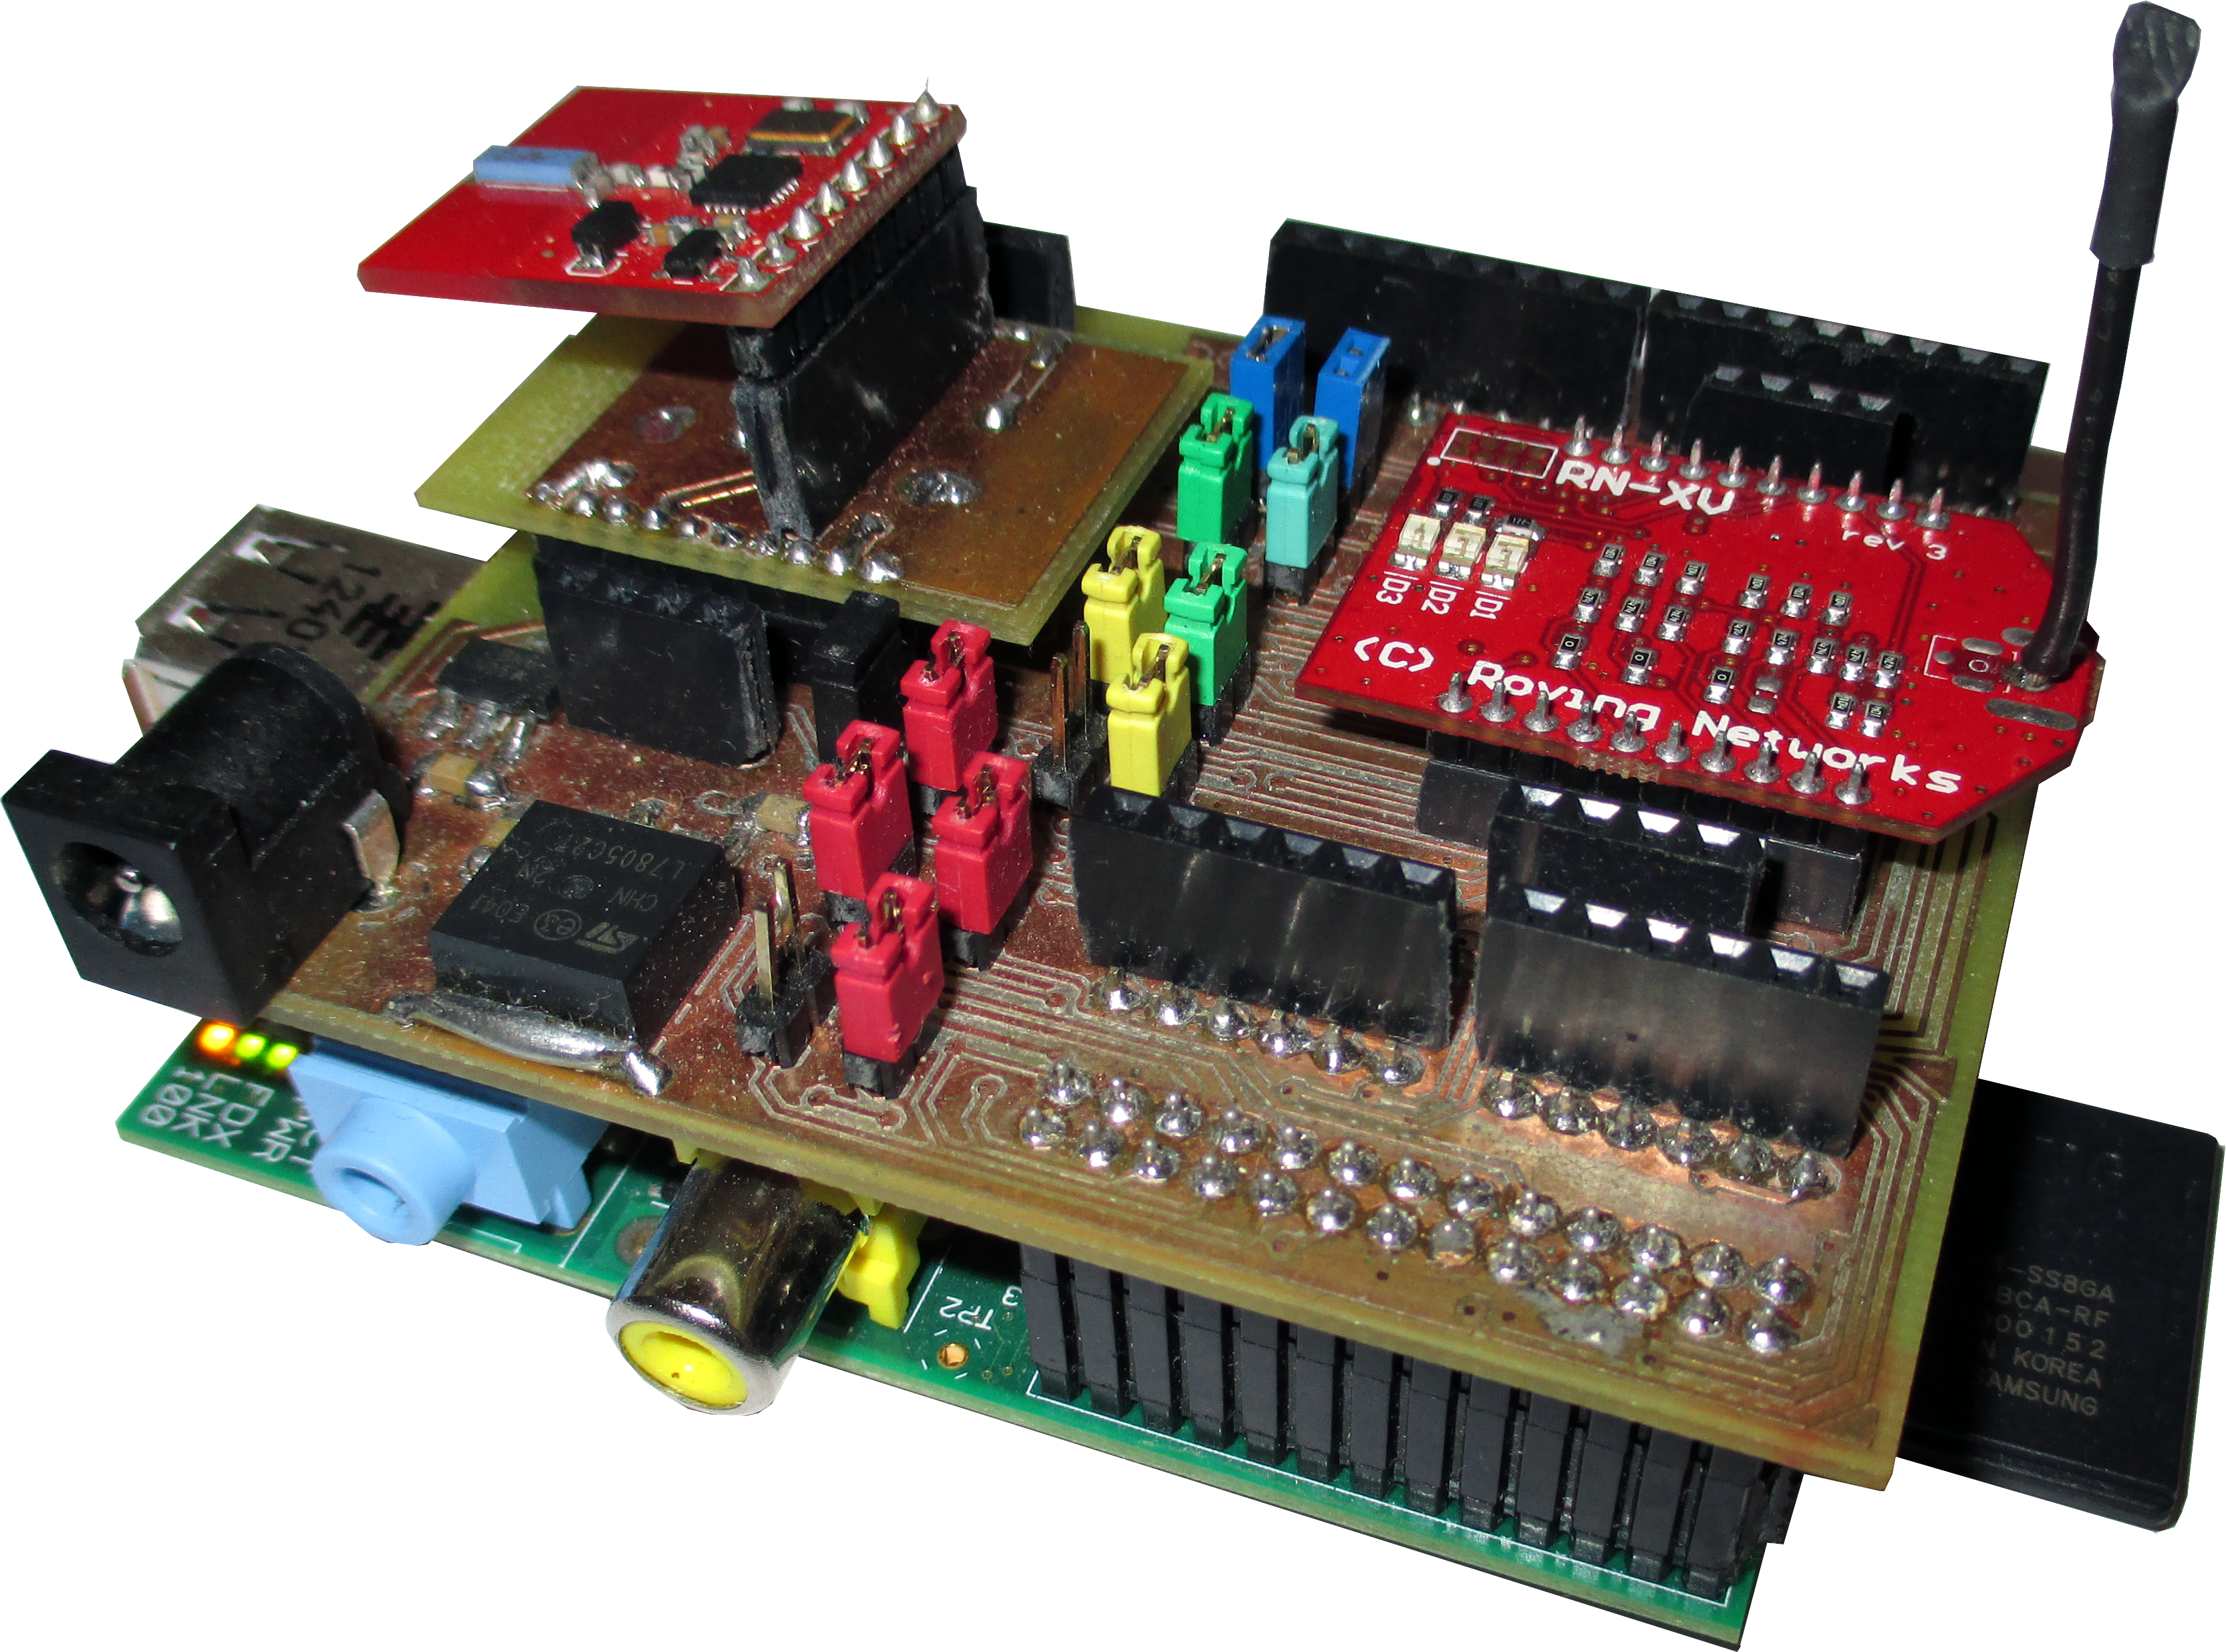
\includegraphics[width=0.6\textwidth]{pictures/examples/raspihomestack}
  \caption{Raspberry Pi with the modules needed to run HomeSense\label{fig:IOEx-HS-Stack}}
\end{center}\end{figure}

\subsection{Working}\label{SS:IOEx-HomeSense-Working}
As IOSharp has implemented all the features required in HomeSense it is possible to change the project type from Micro Framework to .NET Framework and then reference this project. Finally the ports need to be remapped according to the shield used with the Raspberry Pi. The strategy to do this mapping is include the Hardware class of the Raspberry Pi and then rename the ports to the according ones. SerialPort device also must be renamed from \verb!COM1! to \verb!/dev/ttyAMA0!. After changing the references and the port names is possible to start testing the program. So it has been really easy to migrate from the Netduino Mini to the Raspberry Pi.
\\
\\
HomeSense has a program which shows the network status with its gateway and the different sensors connected to the network. On the following figure is shown the scenario. The aaaida logo represents the gateway whereas the node is represented by a door. In this case, both are linked as an arrow connects both of them. With this program is possible to know the network addresses of both devices. Also it shows other information like battery state or the fetched information by any sensor located on a node.
\begin{figure}[H]\begin{center}
 \centering
  \captionsetup{justification=centering}
  \includegraphics[width=1\textwidth]{pictures/examples/homesense-pillin}
  \caption{HomeSense dashboard. The aaaida logo on the left represents the Raspberry Pi (gateway)  whereas the door represents a sensor\label{fig:IOEx-HS-Dash}}
\end{center}\end{figure}

\section{Conclusions}\label{S:Results-overview}
All the functional tests show that IOSharp has been successfully done. Each test works on the Raspberry Pi with doing only minor changes on the code. With IOSharp working and being able to be used on existing Micro Framework projects to make them run on other platforms the development milestone has been done. But, after testing the different parts of IOSharp and deploying HomeSense on the Raspberry Pi using Mono it was seen that the performance was not as good as it was expected. Raspberry Pi, need more time to send the network events than the Netduino and this is probably related to the time needed to attend the interruptions on Mono. In this case the IOSharp with Mono needs two transmissions to send the same information that is send with only one transmission using the Netduino.
\\
To try to solve these issues with the performance of the library, IOSharp will be translated to C++ using a translating tool called AlterNative which is capable of translate .NET assemblies to C++ while maintaining a similar C\# syntax.
\chapter{AlterNative}\label{C:AlterNative}
This chapter is a walk-through AlterNative explaining its concept, how translates the code, then an example using IOSharp will be used along with some use cases that can be applied to this tool.
\section{Concept}\label{S:AN-Concept}
The concept of AlterNative is to maximize the idea of Internet of Things by providing a tool to port applications from high-level languages (such as .NET) to native languages (such as C++) easily. Most of the actual systems are C++ compatible, thus if the application is ported to this language, it can be executed in several platforms (i.e. smartphones, tablets, embedded systems, computers with different operating systems).
\\
With this tool a developer can take the advantages of fast developing in a high-level languages such as C\# and then gain the advantage of performance related the low-level languages like C++. Apart from this it also gives the possibility to get native code capable of work in several systems, in other words, this philosophy is similar to the WORA (Write Once, Run Anywhere) slogan created by Sun Microsystems to illustrate the cross-platform benefits of Java Virtual Machine. The difference is that AlterNative is focused on the final performance because it outputs the original code in native language and does not depend on any virtual machine.
\section{Process}\label{S:AN-Process}
AlterNative process is divided in three steps: decompilation, translation and recompilation.
To summarize the following sections the figure \ref{fig:AN-Process} shows the process that is done from the original assembly, the decompilation, translation and recompilation to a native assembly.
\begin{figure}[H]\begin{center}
 \centering
  \captionsetup{justification=centering}
  \includegraphics[width=1\textwidth]{pictures/alternative/process}
  \caption{AlterNative process\label{fig:AN-Process}}
\end{center}\end{figure}

\subsection{Decompilation}\label{SS:AN-Process-Decom}
First of all the Assembly (compiled program/binary) is passed through a decompiler in order to extract the source code. In this case the code extracted is C\# and to decompile it is used the ILSpy which is an open-source .NET assembly decompiler. The code is not extracted in text format, but in an AST (Abstract Syntax Tree) that is an abstract representation with nodes and hierarchies of the original code. This representation is organized in a tree from the top-level (Assembly) until de low-level (instructions, types and constants).
\\
\\
The figure \ref{fig:AN-AST} shows how the \verb!void Main(string[] args){}! method would look like in AST format. The top node designates that the child nodes correspond to a method, then in the first row child is described the primitive type (what would return the method) which is \verb!void! in this case, the identifier which shows the method name (\verb!Main!) and finally the parameter declaration which describes the parameters that the function takes. In the method shown in the example has one parameter corresponding to an array of strings. The parameter declaration node has two nodes defining it, the first one describes that \verb!string[]! is a composed type by a string and an array specifier, the second node is the identifier name of the parameter, in this case, \verb!args!.
\begin{figure}[H]\begin{center}
 \centering
  \captionsetup{justification=centering}
  \includegraphics[width=0.7\textwidth]{pictures/alternative/csharp_main_ast}
  \caption{AST representation of the main method in C\#\label{fig:AN-AST}}
\end{center}\end{figure}
The translator will generate the C++ code from the AST representation of the original code.
\subsection{Translation}\label{SS:AN-Process-Translation}
To proceed with the translation it is important to know the how is typed the resulting language, then in order to achieve that some modifications need to be applied to the AST, by doing this a second AST will be obtained representing the source code of the desired language. After doing this conversions the following step is start writing the files containing the text representation of the tree. AlterNative translates the code to C++ so the AST changes must be done in a way that the resulting AST corresponds to that language. When printing the new code the headers and the code files must be printed.
\\
\\
Following the example explained in the previous section now the AST will be transformed to the correspond with the C++ one. In C\# the method was \verb!void Main(string[] args){}! but in C++ the syntax is different because the array specifier moves from the primitive type to the identifier. The figure \ref{fig:AN-AST-Conversions} shows in red the changes done to the original tree to achieve an AST corresponding to the C++ method which looks like \verb!void Main(string args[])!. The original identifier changes to a composed identifier with two child nodes, the first one is the identifier \verb!args! and the second one is the array specifier moved from the original composed type to the composed identifier. As there is no composed type now the node is deleted and the parameter declaration is directly linked to the primitive type string.
\begin{figure}[H]\begin{center}
 \centering
  \captionsetup{justification=centering}
  \includegraphics[width=0.7\textwidth]{pictures/alternative/ast_conversions_cpp}
  \caption{AST representation of the main method in C++\label{fig:AN-AST-Conversions}}
\end{center}\end{figure}

\subsection{Recompilation}\label{SS:AN-Process-Recompilation}
The final step consists on compile the C++ code into a new assembly. This final assembly maintains the same functionalities of the first one but taking the benefits of the performance that gives native code. Although it could seem that this software is focused on the code translation but it is not its real finality because its aim is to maintain all the features of the original code like the garbage collector, specific expressions or even language syntax. With all of this passed through AlterNative the program will run much faster than the original one because it is running in native code.
\\
AlterNative is able to provide most of the features of the original code to the final code using external open-source libraries like the boehm GC for the garbage collector, the boost library for the threading and datetime library and finally a proprietary library which implements all the \verb!System! namespace of C\#. With all of this the final assembly is fully compatible with any system like Windows, Linux, Android or any device capable of execute C++ binaries.

\section{Use Cases}\label{S:AN-Use-Cases}
There are two clearly use cases of AlterNative together with IOSharp, the first one is performance and the second one is generate cross-platform programs for embedded systems.
\subsection{Performance}\label{SS:AN-Use-Cases-Perf}
AlterNative gets the major advantage when is applied to programs or libraries which are very complex in a computational way for example image processing, mathematics or complex algorithms where languages running on virtual machines are not as fast as the developer needs. The more complex is the target, the more benefit that can be obtained.
Taking into account that the performance seen on IOSharp over Mono is not as good as it should be compared to the native Micro Framework with a Netduino. Is supposed that passing a program created with IOSharp (which runs on top of Mono) through the translator will generate a faster binary because it does not depend on a virtual machine , and is well known that Mono is not the fastest implementation of the .NET specification.

\subsection{Cross-Platform in embedded systems}\label{SS:AN-Use-Cases-NETMF}
Other advantage of the standard low level languages like C++ is that a high percentage of device processors can execute this code. And at this point is where fits with the implementation of IOSharp because passing the library through AlterNative a new library will be obtained but instead of being written in C\# it will be in C++. By doing this the generated source can be compiled into an ARM-Linux assembly so the unique requirement to execute that code will be an underlying Linux running on the machine. The developer will get all the benefits of Micro Framework with the speed of C++, the code will be written using IOSharp or native Micro Framework which is really easy to develop embedded applications with this software and then translate the program with AlterNative.

\section{Work done in AlterNative}\label{AN-WorkDone}
To achieve the translation (or partial translation) of IOSharp through AlterNative some work was done on the proprietary implementation of \verb!System! libraries which are the the C++ libraries that externally look like the C\# ones but the methods are implemented using standard C++ functions with the boost library or other libraries like the Boehm GC.
\\
\\
At the beginning AlterNative only worked on Windows because some classes from the ILSpy had mixed some functions for the view and some functions from the decompiler so it was unable to run in Linux because the part of the view could not compile. In order to solve that an AlterNative.Core was created which could work in any system that could run C\# code. This core version has its own solution and csproj file but they are pointed to the same code files of the original program. In this way AlterNative can run either on .NET Framework in Windows or on Mono in Linux and MacOSX.
\\
\\
The first attempt to translate IOSharp was unsuccessful but it helped to determine how much the translation was near to be successful. There where several major features that AlterNative was not able to translate like the threading, the delegates used in the interruptions, the P/Invokes or some functions like DateTime, Timer and file access to read and write. Many of these features need to be implemented on the proprietary library because this is linked to the translated program as C\# does with its own libraries.
\\
To implement this features the C++ boost library has been used. This library uses standard C++ functions so it can work in any device or operating system capable of execute binaries compiled from C++.

\section{Example}\label{SS:AN-Process-Example}
The best example to show in this section will be some of the parts of IOSharp translated to C++. In the moment of writing this thesis the only component working well in the translation was the GPIO ports which basically they use the \gls{SYSFS} of Linux and the interrupt port which uses calls to C is also working.
\\
\\
dfdf
\\
\\
Some performance tests had been carried out to quantify how much is faster the translation of IOSharp compared with the original one running on Mono. The explanation of the tests and its results are on the next chapter.
\chapter{Performance tests}\label{C:Performance-Test}
In this chapter are shown the performance results for two tests carried out on a Raspberry Pi using the original implementation of IOSharp, and the C++ version, which is a direct translation using AlterNative.
\\
Theoretically, C++ has a major performance compared to C\# but this tests will be used to determine how much gains C++  over C\#.
\\
The Logic16 has been used to make the timing measurements. This is a channel analyser used to record, view, and measure digital signals.

\section{Compilation types}\label{S:PERF-comptypes}
When a compiler generates a binary from a source code normally tries to do some changes to optimize some attributes of the program. The most common requirement is to optimize the time taken to execute that program, another one is optimize the amount of memory required by the program. Also, some optimizations can be used to make a program consume less power and this is interesting because nowadays the Internet of Things is growing and many sensors have a small battery so reaching low-power consumption is great because it ensures a longest battery life or at least the sensor can operate more time. All of this optimizations are carried out by a sequence of optimizing transformations and algorithms which are applied by optimizing compilers.
\\
Normally compilers can generate programs optimized or non-optimized, depending on how is configured the build system. If the compiler uses optimizations the compile time will grow but the program will be much more optimized than if optimizations are not applied.
\begin{itemize}
  \item \textbf{Non-optimized or debug:} this mode is used by developers who want to debug applications in execution time. In this case the whole symbol information, which is used by the debugger to stop at the break points (designated instructions), is attached to the generated assembly. For example the \verb!*.pdb! files from Visual Studio are created by the compiler and have the information to debug the created assembly. On the other hand, the debug mode will not allow some optimizations because are incompatible with the debugging functionality.
  \item \textbf{Optimized or release:} this mode is used to generate an optimized assembly to run or perform much faster than the debug one. In this case, the compiler performs different transformations to the original code, for example two typical optimizations that cannot be applied to a debug build are:
  \begin{itemize}
  	\item \textbf{Loop unrolling:} the compiler analyses how many times the loop is executed and then it copies the inner code the same number of times. This helps avoiding the maintenance of the loop variables.
  	\item \textbf{Inlining:} the compiler places the method on the place of the call avoiding the stack overhead produced by a method's call.
  	\begin{lstlisting}[language=C++, caption={Inline example}]
inline int Max(int x, int y)
{
   return (x > y)? x : y;
}
int main( )
{
   int a = 100;
   int b = 1010;
   cout << "Max (a, b): " << Max(a, b) << endl;
   return 0;
}

/* The Max(int, int) function is inlined to the main Max call in the following way:*/
int main( )
{
   int a = 100;
   int b = 1010;
   cout << "Max (a,b): " << (a>b)? a : b << endl;
   return 0;
}
\end{lstlisting}
  \end{itemize}
\end{itemize}

\section{GPIO}\label{SS:IOEx-GPIO}
GPIO test consists on how much time takes the board to perform a certain number of iterations changing an output port between the high and low states. Two channels are used in this test, the first one will activate the Logic16 to start sniffing the second channel which will be the one that performs the changes. 
\\
\\
The following code shows the test using the C\# implementation. This is the minimum test to analyse the performance of Mono and C++ when I/O is involved using the original IOSharp and its translation. In this case, it is measured the whole time that system requires to change the state of an output port in a certain number of iterations.
\begin{lstlisting}[language=CSharp, caption={GPIO Performance test in C\#}]
using System;
using System.Collections.Generic;
using System.Linq;
using System.Text;
using Microsoft.SPOT.Hardware;
using IOSharp.NETMF.RaspberryPi.Hardware;
using System.Threading;

namespace raspberrypi
{
    class Program
    {
        public static void Main()
        {
            Debug.Print("START");
            OutputPort bar = new OutputPort(Pins.V2_GPIO17, false);
            bar.Write(false);
            bool foo = false;
            OutputPort o = new OutputPort(Pins.V2_GPIO11, false);

            bar.Write(true);
            for (int i = 0; i < 10000; i++)
            {
                foo = !foo;
                o.Write(foo);
            }
            bar.Write(false);
            Debug.Print("END");
        }
    }
}
\end{lstlisting}
The following code corresponds to the C++ translation.
\begin{lstlisting}[language=C++, caption={GPIO Performance translated to C++}]
#include "Program.h"
namespace raspberrypi {

	void Program::Main(){
		Program* p = new Program();
		p->Run();
	}

	void Program::Run(){
		Debug::Print(new String("START"));
		OutputPort* bar = new OutputPort(Cpu::Pin::GPIO_Pin17, false);
	
		bar->Write(false);
		bool foo = false;
		OutputPort* o = new OutputPort(Cpu::Pin::GPIO_Pin11, false);
		bar->Write(true);
		for (int i = 0; i < 200; i += 1) {
			Debug::Print(new String(i));
			foo = !foo;
			o->Write(foo);
		}
		bar->Write(false);
		Debug::Print(new String("END"));
	}
}
\end{lstlisting}

This test has been executed varying the number of iterations between 200 and 10000. Each iteration swaps the port state between high and low. Apart from this iteration increase, the assembly is compiled using both compiling modes.

\subsection{200 Iterations}\label{SS:200-iterations}
The result produced by Mono with the optimized assembly shows an irregular pattern consisting of two small pulses followed by a wide pulse, and then two small pulses followed by a wide gap. In the figure \ref{fig:gpio-200it-csharp} this pattern is coloured in blue and as it can be seen, it is regularly repeated across all the test. The wide pulses and gaps are supposed to be caused by the garbage collector and the thread round-robin that Mono does.
\\
The small pulses are around 1 ms and the wide gaps/pulses are 2 ms long. Each block is repeated every 10 ms.
\begin{figure}[H]\begin{center}
 \centering
  \captionsetup{justification=centering}
  \includegraphics[scale=0.35]{pictures/performance-tests/GPIO/200/csharp2}
  \caption{200 Iterations using C\# with optimizations\label{fig:gpio-200it-csharp}}
\end{center}\end{figure}
The figure \ref{fig:gpio-200it-csharp} represents this 200 changes in the output state. The required time to make this iterations is the elapsed time between the marker 1 and the marker 2. The Raspberry Pi with Mono needs 202 ms in order to do all the iterations.
\\
\\
After testing the performance in Mono it was time to try out the code generated by AlterNative, which is also compiled in release mode. The resulting test is shown and explained below.
\begin{figure}[H]\begin{center}
 \centering
  \captionsetup{justification=centering}
  \includegraphics[scale=0.35]{pictures/performance-tests/GPIO/200/cxx}
  \caption{200 Iterations using C++ with optimizations \label{fig:gpio-200it-cxx}}
\end{center}\end{figure}
This above image uses the same scale as the figure \ref{fig:gpio-200it-csharp} shows, so the magnitude of the elapsed time can be compared.
\\
\\
In the case of C++ test, it can be observed that the pulses are much more regular than the Mono test, but at certain point around the pulse 89 a big gap is observed probably due to the lack of a garbage collector (AlterNative programs currently do not have a working garbage collector implemented). It is relevant to remark that C++ needs only 77 ms to perform the same test, and each pulse is 0.43 ms on average.
\\
\\
After doing some tests on debug and release mode in both languages a graphic could be sketched, the performance in 200 iterations on Mono using both compile types was the practically the same, it took around 200 ms to complete all the test, however in C++ the time varies a bit depending on the compilation type, without using optimizations it takes 100 ms but when optimization is applied the time decreases to 78 ms.
\\
From the figure \ref{fig:gpio-graph-200} can be concluded that the C++ version is a 62\% faster than the Mono one.
\begin{figure}[H]\begin{center}
 \centering
  \captionsetup{justification=centering}
  \includegraphics[scale=0.9,page=1]{pictures/performance-tests/GPIO/graphs}
  \caption{Graph showing the elapsed time for the 200 iteration test. Blue is for C++ while orange is C\#. On the left is represented the non-optimized compilations and on the right the optimized ones\label{fig:gpio-graph-200}}
\end{center}\end{figure}

\subsection{10K Iterations}\label{SS:10K-iterations}
After testing the 200 iterations another one was done, but increasing the number of iterations to 10000 or in a factor of fifty. In this magnitude the compiler optimizations should be visible enough to observe some kind of improvement on the different compilation and language types.
\\
In the figure \ref{fig:gpio-10kit-csharp+cpp} is represented the elapsed time for 10k iterations, the block on the left is the Mono version and lasts 10 seconds while the second one is the C++ version and the iterations are done in approximately 3 seconds being approximately three times faster.
\begin{figure}[H]\begin{center}
 \centering
  \captionsetup{justification=centering}
  \includegraphics[width=1\textwidth]{pictures/performance-tests/GPIO/10k/cxx+csharp}
  \caption{10k Iterations using C\# with optimizations \label{fig:gpio-10kit-csharp+cpp}}
\end{center}\end{figure}
As it was done in the previous test a graph has been done comparing the different languages and compilation types.
\begin{figure}[H]\begin{center}
 \centering
  \captionsetup{justification=centering}
  \includegraphics[scale=0.9,page=2]{pictures/performance-tests/GPIO/graphs}
  \caption{Graph showing the elapsed time for the 10k iteration test. Blue is for C++ while orange is C\#. On the left is represented the non-optimized compilations and on the right the optimized ones\label{fig:gpio-graph-10k}}
\end{center}\end{figure}
At this number of iterations, the C++ performs much better than C\# and also it is also possible to see an improvement between the debug and release versions of C++ being the optimized version 741 ms faster than the non-optimized one. And the difference between both languages shows that the C++ is 72\% faster than C\#.

\section{Interrupts}\label{S:Performance-Interruptions}
It was observed that in HomeSense the response time in the sensor events was poor, probably because of the time that Mono takes between the interrupt detection and the response. To analyse the elapsed time between the trigger and the response the following test will be polling events from a pin, when an event occurs another pin will be used in output mode with an active high state.
\\
Like the previous test, the C++ code has been generated using AlterNative so it also will be used to test some special functionalities like the delegates, the thread and the timer. The program will start and then create a delegate which will be the called function when an interrupt occurs.
\\
In the figure \ref{fig:interrupt-csharp} is shown the triggering of the interrupt (the top channel with the falling edge), after 1.326 ms the second channel is activated in state high which represents the interrupt response.
\begin{figure}[H]\begin{center}
 \centering
  \captionsetup{justification=centering}
  \includegraphics[scale=0.65]{pictures/performance-tests/Interruptions/csharp}
  \caption{Response time of an interrupt in C\# and Mono\label{fig:interrupt-csharp}}
\end{center}\end{figure}
Then the same test is performed using the C++ version. The result is pretty good because the interrupt is attended only 0.879 ms after the triggering. This implies that C++ is 447 $\mu$s faster than C\#.
\begin{figure}[H]\begin{center}
 \centering
  \captionsetup{justification=centering}
  \includegraphics[scale=0.65]{pictures/performance-tests/Interruptions/cxx}
  \caption{Response time of an interrupt in C++\label{fig:interrupt-cxx}}
\end{center}\end{figure}
It is important to remark that the interrupts in operating systems cannot be considered real-time interrupts, this implies that sometimes an event is attended at a certain time but in another moment, the time required can be much more different due to the non real-time kernel that usually Linux uses. If a hard real-time is needed it is recommended to use other platforms like FreeRTOS which is intended to do tasks that require controlled response times.

\section{Conclusions}\label{S:PerformanceTests-Conclusions}
The iteration test is important because in embedded systems the highest speed that can achieve a board is related to the maximum rate that the board can interact with external devices. Whereas the interrupt test, which analyses the interrupt-response time, is useful to determine the response delay in front of an interrupt. Apart from this, these tests can certify that one of the use cases of AlterNative is real, because the performance is increased as the 10K iteration example shows being 75\% faster than the program running in Mono.
\chapter{Conclusions}\label{C:Conclusions}
\section{Project Conclusions}\label{S:Project-Conclusions}
An implementation of Micro Framework has been done with the necessary features to make the existing software work on it (HomeSense and the RFID card reader). Although it works well the performance is not as good as the original probably because the Micro Framework runs on dedicated hardware and all the consuming operations are implemented internally on the machine so this is the reason why HomeSense works better on the Netduino than on the Raspberry Pi although the second one is much more powerful than the first one.
\\
\\
Another of the goals was create a portable implementation, IOSharp is implemented using C\# and with calls to Linux SYSFS or Kernel functions so this is way this implementation is architecture independent being capable of run either on a standard desktop or on  an ARMv6 like the Raspberry Pi. The only requirement is Linux running under the Mono interpreter.
\\
\\
In order to improve the performance of IOSharp it was translated to C++ using the AlterNative translating tool. Actually it can partially transform the original code to C++ but it still needs a lot of work on its behind because many classes are unimplemented yet. The parts that AlterNative could not translate well where fixed by hand. After all, once IOSharp is translated to C++ the performance gets increased as it is shown in the chapter \ref{C:Performance-Test}. For example in 10000 iterations of a GPIO the C\# implementation needs around 10 seconds to finish while the translated version only spends around 3 seconds, this implies a really big performance compared with the original one.
\\
\\
And finally the best of AlterNative is that the code generated is still cross platform because it uses standard C++ or libraries which are also available on different platforms, so once the source is generated it can be taken to an ARM Linux and compiled to an executable assembly.

\section{Personal Conclusions}\label{S:Personal-Conclusions}
Beyond academic achievements, all the process involving this bachelors thesis has been rewarding. This project has given me a real chance to start working with embedded virtual machines, protocols to communicate hardware modules and also it has provided an introduction to C++ development and code transformations.
\\
\\
This project has allowed me to get familiar with Micro Framework and Linux development, which represents the new paths for the embedded systems where the resource-constrained devices begin to implement Linux kernels to make easy the development of applications. Then on the AlterNative part of the project an introduction to AST pattern was done together with C++ development focused on multi-platform environments. 
\\
\\
There are many skills acquired or consolidated during this time: from the initial touchdown on Micro Framework, platform invocation services to do cross language calls, delegation patterns, guidelines for application performance, etc.
\\
\\
I also have realized that the development of a project is a quite complex task and requires hard effort and dedication, but most of all a strict control of timings in order to accomplish with the established work plan.
\\
\\
In addition, the experience working with my tutor has been very positive too, because he leave so much leeway. The direct and close communication with him, has allowed me to fulfil with the objectives and deadlines.

\section{Future Work}\label{S:Future-Work}
The results of this bachelors thesis point to several interesting directions for future work.
In case of the IOSharp implementation of Micro Framework:
\begin{itemize}
\item \textbf{Addition of new protocols:} Currently IOSharp offers the simple GPIOs, UART and SPI but there are other common protocols or interfaces that could be developed to extend the features such as the \gls{I2C} bus protocol. It will also be nice to implement the analogical ports or even \gls{PWM} control in I/O ports.

\item \textbf{Performance optimization:} The implementation in .NET is too much slow running on Mono, probably related to the use of the \gls{SYSFS}. It could be interesting to do some performance tests using the \gls{SYSFS} or the Kernel functions provided by Linux. Apart from this, the interruptions are not implemented using \gls{IRQ} so try to change from polling to \gls{IRQ} interruptions could be a good improvement on performance but one of the cons of this implementation could be the portability between boards, some distributions do not accept IRQ interruptions from the GPIOs.

\item \textbf{Extend capabilities:} It could be interesting to make IOSharp work with MAREA2 which is a Middleware for distributed embedded systems in different areas like: telecommunications, avionics, health-care, automotive, defense, etc. MAREA is a software specifically designed to fulfil Unmanned Aircraft Systems (UAS) communications and their application to the
design of complex distributed UAS avionics.

\end{itemize}

In case of the AlterNative translation tool:
\begin{itemize}
\item \textbf{Garbage Collector:} Although AlterNative have a garbage collector implemented using the Boehm GC library it does not get called periodically so programs with a big footprint in RAM can get out of memory because this is not freed until the end of the program execution.

\item \textbf{Continuous Integration:} Changes on the core or the libraries of AlterNative are very susceptible to break some implemented functionalities, this is why the regression tests where created to test if the different functionalities are working well. The problem is that this test takes a huge amount of time to finish so using continuous integration tools such as Jenkins or Hudson can provide an easy way to quickly test this changes on a server capable of detect new commits to a git repository. After executing all the test an inform can be mailed to know if all is working fine.
\end{itemize}
\section{Environmental Impact}\label{S:Environmental-Impact}
At last but not least it is necessary to talk about the environmental impact of the work
described in this document. As can be seen from the present document, this project
consists in the design and development of a software application. This has not a direct
environmental benefit, but IOSharp was an implementation on a high-level basis of .NET Micro Framework which is an operating system for embedded devices, so it makes easy to develop applications which helps control from home installations (i.e. lights, temperature or humidity) to applications capable of detect and analyze different parameters from the environment (i.e. weather stations).
%% Remove the final dot and print the glossaries
%\renewcommand*{\glspostdescription}{}
\printglossaries

%%%%%%%%%%%%%%%%%%%%%%%%%%%%%%%%%%%%%%%%%%%%%%%%%%%%%%%%%%%%%%%%%%%%%%%%%
%%%  BIBLIOGRAFIA
%%%%%%%%%%%%%%%%%%%%%%%%%%%%%%%%%%%%%%%%%%%%%%%%%%%%%%%%%%%%%%%%%%%%%%%%%%

%%% Per la bibliografia hi ha 2 opcions: generarla amb la utilitat BibTeX 
%%%                                      o fer-la ''a ma''
%%% NOTA: podeu trobar facilment informaci� sobre BibTeX a:
%%%  http://www.ctan.org/tex-archive/biblio/bibtex/contrib/doc/


%%% OPCIO 1: BibTeX -> descomentar les dues l�nies
%%% a)  Estil de bibliografia\\
%\bibliographystyle{unsrt}  
%%% b) Indicar els fitxers que contenen la bibliografia
%\bibliography{bibliography2}  

%%% OPCIO 2: bibliografia manual
%%%
%%% L'argument d'entrada es el numero de referencies que s'inclouen
\renewcommand{\bibname}{REFERENCES}
\begin{thebibliography}{9}

%% Llibres:  Autor/s (cognoms i inicials dels noms), t�tol del llibre (en cursiva), editor, ciutat i any de publicaci�. Quan es cita el cap�tol d'un llibre s'ha d'indicar el t�tol del cap�tol (entre cometes), el t�tol del llibre (en cursiva) i els n�meros de p�gines amb la primera i la darrera incloses.
%%  Exemple de capitol en llibre

\bibitem{cite:sensors-everywhere}
G�mez, C., Paradells, J. and E. Caballero, J, "Operating Systems", {\it Sensors Everywhere. Wireless Network Technologies and Solutions}, p.273-278, Fundaci�n Vodafone Espa�a, 2010. Also available at \url{http://fundacion.vodafone.es/static/fichero/pre_ucm_mgmt_002618.pdf}

\bibitem{cite:mom}
Bagula, A.B., Denko, M.K. and Zennaro, M., "Middleware for Mobile and Pervasive Services", Chap. 7 in {\it Handbook of mobile systems applications and services}, Taylor and Francis Group, Kumar, A. and Xie, B., pp. 248-249, Boca Raton (FL), 2012. 

\bibitem{cite:oom}
Khan, S., Qureshi, K. and Rashid, H., "Performance Comparison of ICE, HORB, CORBA and Dot 
NET Remoting Middleware Technologies", {\it International Journal of Computer Applications}, 3(11), 15-18 (2010). Also available at \url{http://www.ijcaonline.org/volume3/number11/pxc3871105.pdf}

\bibitem{cite:marea}
L�pez, J., Royo, P., Barrado, C., Pastor, E., "Applying marea middleware to UAS communications", {\it  In Proceedings of the AIAA Infotech@Aerospace Conference and AIAA Unmanned Unlimited Conference 2009}, Seattle (WH). Also available at \url{http://upcommons.upc.edu/e-prints/bitstream/2117/9248/1/infotech09.pdf}

\bibitem{cite:thesis-soa-avionics}
L�pez, J., "Service Oriented Architecture for Embedded (Avionics) Applications", {\it  The PhD Program on Computer Architecture Technical School of Castelldefels Technical University of Catalonia}, Barcelona, 2011. Also available at \url{https://dl.dropbox.com/u/2857619/thesis-small.pdf}

\bibitem{cite:delegate}  
Kiely, D., "Delegates Tutorial" in {\it The Microsoft Developer Network (MSDN)}. Available at \url{http://msdn.microsoft.com/en-us/library/aa288459(v=vs.71).aspx}

\bibitem{cite:serialization} 
Albahari, J. and Albahari B., "Serialization", Chap. 17 in {\it C\# 5.0 in a Nutshell: The definitive reference},
O`REILLY, Roumeliotis, R., pp. 691-728, Sebastopol (CA), 2012.

\bibitem{cite:performance-sockets} 
Kiely, D., "Get Closer to the Wire with High-Performance Sockets in .NET" in {\it The Microsoft Developer Network (MSDN) Magazine}. Available at \url{http://msdn.microsoft.com/es-es/magazine/cc300760(en-us).aspx}

\bibitem{cite:backporting}
Books Llc, Source Wikipedia, "Software Quality: Software Crisis, Kludge, Second-System Effect, Workaround, Reliability Engineering, Fault-Tolerant System", Books Llc, Memphis (Tennessee), 2011.

\end{thebibliography}

%%%%%%%%%%%%%%%%%%%%%%%%%%%%%%%%%%%%%%%%%%%%%%%%%%%%%%%%%%%%%%%%%%%%%%%%%%
%%%%%%                           APENDIXS                         %%%%%%%%
%%%%%%%%%%%%%%%%%%%%%%%%%%%%%%%%%%%%%%%%%%%%%%%%%%%%%%%%%%%%%%%%%%%%%%%%%%

\pagestyle{empty}  % no tocar

%% Descomentar una de les dues l�nies seg�ents, en funci� de:
%%  a) els apendixs s'encuadernaran apart (amb portada) 
%%  b) els apendixs s'enquadernen amb el mateix projecte (sense portada). 
%% Recordeu que si tot el document (amb ap�ndixs) excedeix les 100 pagines 
%% s'ha d'enquadernar a part
\appendix\ambportada
%\appendix\senseportada


%%%%%%%%%%%%%%%%%%%%%%%%%%%%%%%%%%%%%%%%%%%%%%%%%%%%%%%%%%%%%%%%%%%%%%%%%%
%%%%%% INCLOURE A PARTIR D'AQUI TOTS ELS CAP�TOLS DELS APENDIXS   %%%%%%%%
%%%%%%%%%%%%%%%%%%%%%%%%%%%%%%%%%%%%%%%%%%%%%%%%%%%%%%%%%%%%%%%%%%%%%%%%%%
\chapter{Tools}\label{C:Tools}

\section{Source control tools}\label{S:Tools-control}
\subsection{Git}\label{SS:Tools-Git}
\subsection{GitHub}\label{SS:Tools-GitHub}
\subsection{Git source control provider extension}\label{SS:Tools-GitSource}

\section{Package management system}\label{S:Tools-pms}

\subsection{NuGet}\label{SS:Tools-NuGet}

NuGet is a free, open source developer focused package management system for the .NET platform intent on simplifying the process of incorporating third party libraries into a .NET application during development.

\subsection{Packages}\label{SS:Tools-packages}

\subsubsection{Log4net}\label{SSS:Tools-log4net}

Log4net, a port of the popular Java library log4j, is an open source library that allows .NET applications to log output to a variety of sources (e.g., console, files or SMTP). The information is logged via one or more loggers which provide a the following five logging levels: 

\begin{itemize}
\item \textbf{Debug}   
\item \textbf{Information} 
\item \textbf{Warnings}
\item \textbf{Error} 
\item \textbf{Fatal} 
\end{itemize}

\subsubsection{NUnit}\label{SSS:Tools-Nunit}

NUnit, a port from JUnit, is a unit-testing framework for all .NET languages. It is written entirely in C\# and has been completely redesigned to take advantage of many .NET language features, for example custom attributes and other reflection related capabilities. 

NUnit does not support Visual Studio integration. Instead of this it provides an external program compiled either as a console app or a GUI. This program is able to runs and execute the unit tests from an assembly.

\begin{figure}[H]\begin{center}
 \centering
  \captionsetup{justification=centering}
  \includegraphics[scale=0.45]{pictures/appendices/tools/NuGetGUI}
  \caption{MAREA unit tests executed by NUnit GUI application\label{fig:tools-NUnitGUI}}
\end{center}\end{figure}

This framework has been especially used to test encoder layer functionalities. The listing \ref{lst:NUnit-test} shows an example of a unit test to serialize and deserialize a double with two diferent pair of parameters.

\begin{lstlisting}[language=CSharp, caption={MAREA encoder layer unit test: serialization and deserialization of a double}, classoffset=2,morekeywords={SetUp,TestCase,PerformanceTimer,ResultsManager,Description,AdaptedMareaCoder,CoderTestsConstants,Results,Console,Assert},label={lst:NUnit-test}]
 private byte[] seralizedData = null;
 private long start, serializeTicks, deserializeTicks;
 private long  clock_freq = PerformanceTimer.Clock_freq();
  
 [SetUp]
 public void RunAfterAnyTest()
 {
  serializeTicks = 0;
  deserializeTicks = 0;
 }
  
 [TestCase(0.100000234523, 0), NUnit.Framework.Description("Coder(double, System.Double)")]
 [TestCase(double.MaxValue,0)]
 public void TestDoubleM2(double oDouble, double rDouble)
 {
  for (int i = 0; i < CoderTestsConstants.CODIFICATIONS; i++)
  {
   start = PerformanceTimer.Ticks();
   seralizedData = AdaptedMareaCoder.Send(oDouble);
   serializeTicks += PerformanceTimer.TicksDifference(start);

   start = PerformanceTimer.Ticks();
   rDouble = (double)AdaptedMareaCoder.Receive(seralizedData);
   deserializeTicks += PerformanceTimer.TicksDifference(start);
  } 

  Console.WriteLine(CoderTestsConstants.MAREA2);
  Results results = ResultsManager.GetResults(serializeTicks, deserializeTicks, clock_freq, 				
  CoderTestsConstants.CODIFICATIONS, seralizedData.Length, rDouble.GetType().FullName);
	
  if (oDouble == rDouble)
  {
   Assert.True(true);
   Console.WriteLine(CoderTestsConstants.OK_STATE);
   Console.WriteLine(results.ToString());
  }
  else
  {
   Console.WriteLine(CoderTestsConstants.KO_STATE);
   Assert.True(false);
  }
 }
\end{lstlisting}

\subsubsection{Nuget Server}\label{SSS:Tools-NuGet-server}

\section{Cross platform tools}\label{S:Tools-control}
\subsection{Mono}\label{SS:Tools-Mono}
\subsection{Alter Native}\label{SS:Tools-Alternative}










%%%%%%%%%%%%%%%%%%%%%%%%%%%%%%%%%%%%%%%%%%%%%%%%%%%%%%%%%%%%%%%%%%%%%%%%%%

%%%%%%%%%%%%%%%%%%%%%%%%%%%%%%%%%%%%%%%%%%%%%%%%%%%%%%%%%%%%%%%%%%%%%%%%%%
%%%%%%%%%%%%%%%%%%%%%%%%%%%%%%%%%%%%%%%%%%%%%%%%%%%%%%%%%%%%%%%%%%%%%%%%%%
%%%%%%%%%%%%%%%%%%%%%%%%%%%%%%%%%%%%%%%%%%%%%%%%%%%%%%%%%%%%%%%%%%%%%%%%%%
% i  aixo es tot! ;)
\cleardoublepage
\end{document}





